\documentclass[11pt, oneside]{article}    % use "amsart" instead of "article" for AMSLaTeX format
\usepackage{geometry}                % See geometry.pdf to learn the layout options. There are lots.
\geometry{letterpaper}                    % ... or a4paper or a5paper or ... 
%\geometry{landscape}                % Activate for rotated page geometry
%\usepackage[parfill]{parskip}    % Activate to begin paragraphs with an empty line rather than an indent
\usepackage{graphicx} % Use pdf, png, jpg, or eps§ with pdflatex; use eps in DVI mode
% TeX will automatically convert eps --> pdf in pdflatex 
\usepackage{amssymb}
\usepackage[T1]{fontenc}
\usepackage[utf8]{inputenc}
\usepackage{authblk}
\usepackage{amsmath} %amsthm, amssymb, amsfonts
\usepackage{subcaption}
\usepackage{float}


%SetFonts

%SetFonts


\title{  MODELING THE EFFECTS OF DRUGS OF ABUSE ON HIV INFECTIONS WITH TWO VIRAL SPECIES}
\author[1]{Peter M. Uhl}
\author[1,2]{Naveen K. Vaidya}
\affil[1]{Computational Science Research Center, San Diego State University}
\affil[2]{Department of Mathematics and Statistics, San Diego State University}
%\date{} % Activate to display a given date or no date

\begin{document}
\maketitle
%\section{}
%\subsection{}

\begin{abstract}

Injection drug use is one of the greatest risk factors associated with contracting human immunodeficiency virus (HIV), and drug abusers infected with HIV suffer from a higher viral load and rapid pathogenesis. Replication of HIV may result in a large number of mutant viruses that can escape recognition of the host’s immune response. Experimental results have shown that the presence of morphine can decrease the viral mutation rate and cellular immune responses. In this study, we present a mathematical model to determine if the decrease in mutation and cellular immune response in the presence of morphine can account for the increased viral load. Two viral species are considered: a wild-type and a mutant. The morphine-altered mutation rate and cellular immune response is shown to allow the wild-type virus to out compete the mutant, resulting in a higher set point viral load. Calculation of the basic reproduction number for each species shows that the dominant species is determined by a threshold morphine concentration, with the mutant dominating below the threshold and the wild-type dominating above. Stability analysis is performed on the infection free and mutant only equilibria of the system and numerical simulations reflect the increased viral load associated with morphine use.

\end{abstract}

\section{Introduction}

	Human immunodeficiency virus (HIV) is a significant health concern in the United States and around the world, with about $56,000$ new infections per year in the United States \cite{MMWR}. HIV is a blood borne pathogen and one of the most common forms of transmission is by the sharing of needles used for injecting drugs of abuse, such as opiodes, between infected and non- infected persons. Drugs of abuse have been shown to have adverse effects on the progression of HIV infections, including a higher set point viral load and decreased amounts of CD4+ T cells \cite{Kumar}. Studies involving rhesus macaques and simian immunodeficiency virus (SIV and HSIV) have shown that morphine causes a faster progression to AIDS and a higher pathogenesis in affected animals, many other studies of HIV have also demonstrated that a quicker progression to AIDS maybe associated with opiate use \cite{Hauser}. It is therefore important to investigate the mechanisms by which morphine affects the progression of HIV infections and viral burden.

\vspace{5mm}

	Cytotoxic T-lymphocytes (CTLs) are an important component of the human immune system for combating viral infections, including HIV, by limiting viral reproduction and the infection of hosts’ target cells. In the acute stage of the infection the host’s immune system responds by creating a large amount of virus specific CTLs. The CTLs perform actions to inhibit viral growth, for example by destroying infected cells directly. After the infection has progressed and the immune response by CTLs has been reduced it is possible for mutant viruses to revert back to the original wild-type strain. Therefore the production of CTLs plays a significant role in the progression of an infection \cite{Greenough}. However, HIV possesses a high genetic variability which results in the production of escape mutants that can avoid detection by CTLs \cite{Boutwell}. The high number of CTLs puts pressure on the virus to quickly mutate to a form that can evade the CTLs, this combined with the quick replication speed of HIV results in a large number of mutant viruses being produced \cite{Deng, Ribeiro}. The production of mutant viruses can be a significant barrier to the treatment of HIV by antiviral drugs or to the development of an effective vaccine \cite{Boutwell}.

\vspace{5mm}

 %Continuous infection of target cells also results in a large amount of newly infected cells and free virus particles \cite{Perelson}.

	

	%The target cells of HIV are CD4+ T cells, which are a part of the immune system that signal other immune cells to attack foreign antigens when they are present \cite{Kitchen, Killeen}. HIV virions attack CD4+ cells by attaching to receptors on the CD4+ cell surface and entering the interior of the cell, where the virions can begin reproducing \cite{Chan}. Once the virus has entered a target cell, the target cell becomes infected and begins releasing new virions. The early stages of infection are characterized by a rapid production of a large number of virions and infected cells \cite{Fauci}, making the early weeks of infection crucial in determining the long-term viral dynamics.

	%In the acute stage of the infection the host’s immune system responds by creating a large amount of virus specific CTLs. The CTLs perform actions to inhibit viral growth, for example producing cytokines that limit viral reproduction, reducing the amount of receptors available on target cells, and by destroying infected cells directly, but it is not clear which actions are the most important for combating acute HIV infections \cite{McMichael}. The high number of CTLs puts pressure on the virus to quickly mutate to a form that can evade the CTLs, this combined with the quick replication speed of HIV results in a large number of mutant viruses being produced \cite{Deng, Ribeiro}. After the infection has progressed and the immune response by CTLs has been reduced it is possible for mutant viruses to revert back to the original wild-type strain.

	Experimental studies have shown that opiates can increase viral replication by increasing CCR5 expression in target cells \cite{Li} and studies on rhesus macaques have shown similar levels of viral growth in the early stages of infection between morphine dependent and control animals, but higher set point viral loads associated with morphine use \cite{Kumar}. Morphine has also been shown to affect the amount of escape mutants that evolve, but the exact effect remains unclear \cite{Noel1}. Mathematical models have been very useful in understanding the dynamics of infectious diseases \cite{Perelson, Chubb}. A problem on which there has been little study is to determine the effects of morphine on the viral dynamics of HIV when multiple viral species are present, and the objective of this paper is to present such a model. Thus, it is desirable to develop a mathematical model that will include components for the host’s cellular immune response (CTLs), escape mutations, and morphine use.

\section{Method}
\subsection{Model}

	The model can be written as the following system of differential equations:

\begin{align*}
T_l' & =  \lambda + q(M) T_h - r(M) T_l - \beta_l V_w T_l - (1-F) \beta_l V_m T_l - \delta_T T_l \\
T_h' & =  r(M) T_l - q(M) T_h - \beta_h V_w T_h - (1-F) \beta_h V_m T_h - \delta_T T_h\\
V_w' & =  p I_w - \delta_V V_w\\
V_m' & =  p I_m - \delta_V V_m\\
I_w' & =  (1-\frac{\epsilon}{\mu + \eta M})(\beta_l V_w T_l + \beta_h V_w T_h) - b I_w C - \delta_I I_w\\
I_m' & = \frac{\epsilon}{\mu + \eta M}(\beta_l V_w T_l + \beta_h V_w T_h) + (1-F) (\beta_l V_m T_l +\beta_h V_m T_h) -\frac{b} {1+B} I_m C -\delta_I I_m\\
C' & =  \omega + \frac{\alpha}{\gamma + \xi M}(I_w + I_m)C - \delta_C C\\
\end{align*}

where $T_l$ and $T_h$ denote target cells, $V_w$ and $V_m$ are wild-type and mutant virus, $I_w$ and $I_m$ are cells infected by the wild-type and mutant virus, respectively, and $C$ is CTLs. Two populations of target cells are included to model the increased susceptibility of some target cells caused by morphine use, so that $T_h$ represents cells that are exhibiting increased co-receptor expression and are more likely to become infected than cells in the $T_h$ population \cite{Vaidya}. Two viral species are included to model the evolution of the virus, so that a portion of cells infected by the wild-type virus undergo mutation and go into the $I_m$ population \cite{Konrad}. The host's cellular immune response is modeld by the population of CTLs, the production of which is stimulated by the presense of infected cells \cite{Konrad}.

\vspace{5mm}

It is assumed that all newly created target cells belong to the $T_l$ population and are produced at rate $\lambda$, and that target cells transision from $T_l$ to $T_h$ at rate $r$ and from $T_h$ to $T_l$ at rate $q$ \cite{Vaidya}. Cells in the $T_l$ population are infected by the wild-type virus at the per capita rate of $\beta_l$ and by mutant virus at per capita rate $(1-F) \beta_l$, where $F$ is the fitness cost of the mutation. Similarly, $T_h$ cells are infected at rates $\beta_h$ and $(1-F) \beta_h$. Both populations of target cells die at $\delta_T$ \cite{Perelson, Schwartz}. 

\vspace{5mm}

Both species of virus proliferate at rate $p$ in proportion to the amount of target cells and are cleared at rate $\delta_V$ \cite{Konrad}. Due to mutation, a fraction $\epsilon$ of target cells infected by wild-type virus become mutant infected cells and the remainder, $(1-\epsilon)$ become wild-type infected cells \cite{Konrad}. Wild-type infected cells are cleared by CTLs at rate $b$. Due to responses by epitope-specfic CTLs there is some recognition of the mutant by CTLs \cite{Konrad,Barouch}, so the clearance rate of the mutant virus by CTLs is modeld by $\frac{b}{1+B}$, where $1+B$ is the escape ratio- a reduction in the ability of CTLs to kill mutant infected cells. Infected cells die at per capita rate $\delta_T$. CTLs are produced at constant rate $\omega$, die at rate $\delta_C$, and are also produced at rate $\alpha$ in proportion to the total number of infected cells, $I_w + I_m$ \cite{Konrad}.

\vspace{5mm}

The effect of morphine on these dynamics will be modeled through three mechanisms: the increase in the $T_h$ population, the decrease in mutation, and the decrease in CTL producution. Morphine changes the rates of transition between target cell populations, giving $q(M)$ and $r(M)$, by decreasing $r(M)$ and decreasing $q(M)$ resulting in more target cells in the $T_h$ population \cite{Vaidya}. This is modeled using an e-max model of the form

\begin{align*}
r(M) &= r_c + (r_m - r_c) \eta_r(M)\\
q(M) &= q_m + (q_c - q_m) \eta_q (M)\\
\end{align*}

where 

\begin{align*}
\eta_r(M) &= \frac{M^n}{M_h^n + M^n}\\
\eta_q(M) &= 1- \eta_r(M).\\
\end{align*}

\vspace{5mm}

The decrease in viral mutation brought on by morphine is modeled by introducing parameters $\mu$ and $\eta$ and reducing $\epsilon$ in proportion to the concentration of morphine, $M$, so that the mutation rate in the presence of morphine is $\frac{\epsilon}{\mu + \eta M}$. Similarly, the decrease in CTL production can be modeled by introducting parameters $\gamma$ and $\xi$ so that the CTL production in response to infection is $\frac{\alpha}{\gamma + \xi M}$ when morphine is present. Finally, the constant rate of CTL production is assumed to decrease exponentially with decay rate $\psi$ when morphine is presnet, so that the new rate of CTL production is $\omega e^{-\psi M}$.


%	Due to different epitote mutations, CTLs are assumed to be produced at constant rate $\omega$ and also to reproduce in the presense of infected cells \cite{Konrad}. Konrad et al. denote $\alpha$ as the rate of CTL production in response to the total amount of infected cells $I_w + I_m$.  The parameters $\gamma$ and $\xi$ are introduced to lower the CTL production rate \cite{Kumar}, changing the CTL produciton rate to $\frac{\alpha}{\gamma + \xi M} (I_w + I_m) C$. CTLs kill wild-type infected cells at rate $b I_w C$, where $b$ is the per capita wild-type clearance rate. Due to responses by epitope-specific CTLs there is some recognition of the mutant by the CTL response \cite{Konrad, Barouch}, so the clearance rate of the mutant virus is assumed to be $\frac{b}{1+B} I_m C$, where $B$ represents the escape ratio- a reduction in the ability of CTLs to kill mutant infected cells. CTLs die at rate $\delta_C C$. Since the viral speices are distinguished only by the fitness cost of the mutant, $F$, and the escape ratio, $B$, it is only neccessary to consider two populations of virus.

	%Deterministic differential equations are used extensively to model infectious disease, and a similar approach will be used here. The simplest HIV model is given by

%\begin{center}
%$\begin{array}{rcl}\label{eq:1}
%T' & = & \lambda - \beta V T - \delta_T T \\
%V' & = & p I - \delta_V V \\
%I' & = & \beta V T - \delta_I I \\
%\end{array}$
%\end{center}

%Where $T$, $I$, and $V$ are the populations of target cells, infected cells, and free virions, respectively, and a prime denotes the derivative with respect to time, in days. Target cells are produced at constant rate $\lambda$ and die naturally at rate $\delta_T$ per cell. Infected cells are produced via the mass action term $\beta T V$ proportional to the number of target cells and free virions. Free virions are produced at rate $p I$ proportional to the number of infected cells. Target cells, infected cells, and free virions die at rates $\delta_T T$, $\delta_I I$, and $\delta_V V$, respectively \cite{Perelson, Schwartz}. 

	%Vaidya et al. \cite{Vaidya} developed a model that incorporates two separate target cell subpopulations based on the experimental observation that morphine can increase the co-receptor expression of certain target cells and make them more susceptible to infection and that individual cells can transition between these subpopulations \cite{Vaidya}. The differential equations for this model are 

%\begin{center}
%$\begin{array}{rcl}\label{eq:1}
%T_l' & = & \lambda + q T_h - r T_l - \beta_l V T_l - \delta_T T_l \\
%T_h' & = & r T_l - q T_h - \beta_h V T_h -  \delta_T T_h \\
%V' & = & p I - \delta_V V \\
%I' & = & \beta_l V T_l + \beta_h V T_h - \delta_I I \\
%\end{array}$
%\end{center}

%The two subpopulations of target cells are denoted $T_l$ and $T_h$ and have corresponding infection terms $\beta_l V T_l$ and $beta_h V T_h$. The subpopulations are distinguished by their different suseptibilities to infection induced by morphine use, with $T_l$ having lower susceptibility and $T_h$ having higher susceptibility. Target cells transistion between subpopulations at rates $ q T_h$ from $T_h$ to $T_l$ and $r T_l$ from $T_l$ to $T_h$.

%	Konrad et al. \cite{Konrad} developed a model to study the effectiveness of a CTL based vaccine that included a wild-type virus $V_w$, a mutant virus $V_m$, and a cellular immune response in the form of CTLs. In their model, the total viral load is divided into subpopulations of wild-type and mutant virus with corresponding subpopulations of infected cells.  This model accounts for immune response by including a population of CTLs, $C$, the production of which is stimulated by the presence of infected cells and which kill infected cells at rates proportional to the populations of CLTs and infected cells.

%Modifying the model from Vaidya et al. \cite{Vaidya} to include populations of wild-type viruses, mutant viruses, and  CTLs results in the system

%\begin{center}
%$\begin{array}{rcl}\label{eq:1}
%T_l' & = & \lambda + q(M) T_h - r(M) T_l - \beta_l V_w T_l - \hat{ \beta_l} V_m T_l - \delta_T T_l \\
%T_h' & = & r(M) T_l - q(M) T_h - \beta_h V_w T_h - \hat{ \beta_h} V_m T_h - \delta_T T_h\\
%V_w' & = & p I_w - \delta_V V_w\\
%V_m' & = & p I_m - \delta_V V_m \label{eq:1}\\ 
%I_w' & = & (1 - \epsilon) (\beta_l V_w T_l + \beta_h V_w T_h) - b I_w C - \delta_I I_w\\
%I_m' & = & \epsilon(\beta_l V_w T_l + \beta_h V_w T_h) + \hat{ \beta_l} V_m T_l + \hat{ \beta_h} V_m T_h \\
%& & -\hat{b} I_m C -\delta_I I_m\\
%C' & = & \omega + \alpha(I_w + I_m)C - \delta_C C\\
%\end{array}$
%\end{center}

%Target cells interact with free virions to produce actively infected cells via infection; target cells are divided into subpopulations $T_l$, which are less susceptible to infection due to lower co-receptor expression, and $T_h$ which are more susceptible to infection. Target cells transition from $T_h$ to $T_l$ at rate $q(M) T_h$ and from $T_l$ to $T_h$ at rate $r(M) T_l$ \cite{Vaidya}, where $q(M)$ and $r(M)$ given by

%\begin{align*}
%r(M) &= r_c + (r_m - r_c) \eta_r(M)\\
%q(M) &= q_m + (q_c - q_m) \eta_q (M)\\
%\end{align*}

%where 

%\begin{align*}
%\eta_r(M) &= \frac{M^n}{M_h^n + M^n}\\
%\eta_q(M) &= 1- \eta_r(M).\\
%\end{align*}

% It is assumed that newly created target cells are all in the $T_l$ subpopulation and are produced at constant rate $\lambda$ \cite{Perelson, Vaidya}. Wild-type virions infect $T_l$ target cells at rate $\beta_l V_w T_l$, where $\beta_l$ is the per capita infection rate of $T_l$ by the wild-type virus. Mutant virions infect $T_l$ target cells at rate $(1-F) \beta_l V_m T_l$, where $F$ is the fitness cost of the mutant virus- a reduction in the mutant's infection rate relative to the wild-type's caused by mutation\cite{Ganusov}. Similarly, $T_h$ cells are infected by wild-type and mutant viruses at rates $\beta_h V_w T_h$ and $(1-F) \beta_h V_m T_h$, respectively, where $\beta_h$ is the per capita infection rate of $T_h$ by the wild-type virus \cite{Konrad}.  Target cells die naturally at rates $\delta_T T_l$ and $\delta_T T_h$ corresponding to $T_l$ and $T_h$, respectively \cite{Smith, Konrad}.

%	When target cells are infected by either the wild-type virus $V_w$ or the mutant virus $V_m$ they become actively infected cells $I_w$ and $I_m$, at which point there is no distinction based on levels of co-receptor expression. In the model developed by Konrad et al \cite{Konrad}, a portion of target cells infected by the wild-type virus mutate and become mutant infected cells rather than wild-type infected cells based on the mutation parameter $\epsilon$. The parameters $\mu$ and $\eta$ are introduced to model the lowered mutation rate caused by morphine \cite{Noel1} so that the per capita mutation rate becomes $\frac{\epsilon}{\mu + \eta M}$, where $M$ is the concentration of morphine which, for simplicity, is assumed to be constant. Therefore, wild-type infected cells are produced at rate $(1 - \frac{\epsilon}{\mu + \eta M})(\beta_l V_w T_l +\beta_h V_w T_h)$, while the remainder $ \frac{\epsilon}{\mu + \eta M}(\beta_l V_w T_l +\beta_h V_w T_h)$ are converted into mutant infected cells. Mutant infected cells are additionally produced by way of infection of target cells by mutant virions at the total rate of $(1-F)(\beta_l V_m T_l +\beta_h V_m T_h)$. Infected cells die at rates $\delta_I I_w$ and $\delta_I I_m$. Wild-type and mutant infected cells produce free virions, $V_w$ and $V_m$, which are cleared at rates $\delta_V V_w$ and $\delta_V V_m$, respectively \cite{Smith, Konrad}.

%	Due to different epitote mutations, CTLs are assumed to be produced at constant rate $\omega$ and also to reproduce in the presense of infected cells \cite{Konrad}. Konrad et al. denote $\alpha$ as the rate of CTL production in response to the total amount of infected cells $I_w + I_m$.  The parameters $\gamma$ and $\xi$ are introduced to lower the CTL production rate \cite{Kumar}, changing the CTL produciton rate to $\frac{\alpha}{\gamma + \xi M} (I_w + I_m) C$. CTLs kill wild-type infected cells at rate $b I_w C$, where $b$ is the per capita wild-type clearance rate. Due to responses by epitope-specific CTLs there is some recognition of the mutant by the CTL response \cite{Konrad, Barouch}, so the clearance rate of the mutant virus is assumed to be $\frac{b}{1+B} I_m C$, where $B$ represents the escape ratio- a reduction in the ability of CTLs to kill mutant infected cells. CTLs die at rate $\delta_C C$. Since the viral speices are distinguished only by the fitness cost of the mutant, $F$, and the escape ratio, $B$, it is only neccessary to consider two populations of virus.



%For simplicity, the notation $\hat{\beta_l} = (1-F) \beta_l$, $\hat{\beta_h} = (1-F) \beta_h$, $\hat{\epsilon} = \frac{\epsilon}{\mu + \eta M}$, and $\hat{\alpha} = \frac{\alpha}{\gamma + \xi M}$ will sometimes be used.  

\subsection{Parameter Estimates}

	Estimates for parameter values are taken from previously published studies. Following Vaidya et al. \cite{Vaidya}, we assume $10^6$ target cells per $ml$ of blood,  about $40980/ml$ belonging to the $T_l$ population and the remaining $10^6 - 40980/ml$ to the $T_h$ population. Since there are initially no infected cells, we take $I_w=I_m = 0$. We estimate the intial viral load $V_0$ based on experimental work. In \cite{Kumar}, rhesus macaques were infected intravenously with 2-ml inoculum containing a cocktail of three SIV viruses. The cocktail contained $10^5$ HIV RNA copies of each of the three viruses, and assuming a macaque contains approximately 1.5 liters of extracellular water we can estimate $V_0 = \frac{3\times 10^5 }{1.5 L} \approx 200$ viral RNA copies/ml \cite{Vaidya}, which we assume belongs entirely to the $V_w$ population. Estimates for $\lambda, \beta_l, \beta_h, r$, and $q$ were taken from Vaidya et al. \cite{Vaidya}, where they were obtained by fitting their model to experimental data. In particular, the observed $\beta_l$ to be approximately two orders of magnitude lower than $\beta_h$. The fitness cost $F$ will vary between 0 and 1.

\vspace{5mm}

	Previous estimates give the average viral clearane rate as 23 cells per day and the average target cell life span as 100 days, so we take $\delta_V = 23$ and $\delta_T = 1/100 = 0.01$ \cite{Ramratnam, Stafford}. We assume only forward-mutation takes place, i.e., that mutant infected cells will not revert to wild-type infected cells, and take the mutation rate as $\epsilon = 3 \times 10^{-5}$ obtained experimentally in \cite{Mansky}. The parameters  $\mu$ and $\eta$ that account for the effect of morphin on $\epsilon$ will vary. Following Konrad, we take the CTL death rate $\delta_C \approx 10^{-1}$ and use the estimate for the CTL production rate $\alpha = 6.7 \times 10^{-5}$ obtained by De Boer and Perelson \cite{Konrad, De Boer}. The parameters $\gamma$ and $\xi$ that account for the effect of morphine on $alpha$ will vary. Previous modeling work by Ganusov gives a range of the CTL killing rate, $b$, between 0.01 and 0.4 \cite{Ganusov} and the escape ratio $B$ will be varied.

\vspace{5mm}

	We assume that the constant rate of CTL production, $\omega$ is 50 cells per day in the absence of morphine and decays exponentially with respect to the morphine concentration, giving $\hat{\omega}(M) = \omega e^{-\psi M}$ with decay rate $\psi$. Olkkola et al measured the kinetics and dynamics of morphine in children and observed initial concentrations of morphine between 28 and 325 $\mu l$ per kilogram of body weight, therefore we will take $M$ between 0 and 300 \cite{Olkkola}.

\vspace{5mm}

	The estimated parameters and their descriptions are summarized in Table 1:

 %They also estimate an initial viral load of $200$ viral RNA copies per $ml$, which is here assumed to all belong to the wild-type population. 

%Since there is initally no infection, $I_w$, $I_m$, and $C$ are all initially zero. Additionally, they estimate  $\lambda$ to be $3690/ml$ per day.  The functions $r(M)$ and $q(M)$ are calculated using $M_h = 2.8534 \times 10^{-3}, r_c = 0.16, r_m = 0.52, q_c = 1.23 \times 10^{-6}, q_m = 0.25, n = 7.8731$ (NEED CITATION). The wild-type infection rate of $T_l$, $\beta_l$, is estimated to be on the order of $10^{-9} ml$ per day and the wild-type infection rate of $T_h$, $\beta_h$ approximately two orders of magnitude higher \cite{Vaiyda}. Finally, they estimate the death rate of infected cells $\delta_I$ as between $0.31$ and $0.78$ cells per day and the common production rate of the viruses as $p = 2500$ (new reference for $p$) virions per day. The infection rates of $T_l$ and $T_h$ by the mutant virus is calculated as a percentage of the corresponding infection rate of the wild-type virus, giving $(1-F) \beta_l$ and $(1-F) \beta_h$ where the fitness cost $F \in [0,1]$ \cite{Perelson}.

	%Ramratnam et al. \cite{Ramratnam} estimate the average virion clearance rate as $23$ cells per day, giving $\delta_V = 23$ \cite{Ramratnam} and Stafford et al. \cite{Stafford} provide the average target cell life span as 100 days, giving $\delta_T = 0.01$ \cite{Stafford}. This model assumes that only forward mutation takes place, i.e., that mutant infected cells will not mutate back into the wild-type infected population. The forward mutation rate $\epsilon$ has been observed experimentally to be $3 \times 10^{-5}$ in \cite{Mansky}, the parameters $\mu$ and $\eta$ that account for the effect of morphine on $\epsilon$ will be varied. De Boer and Perelson \cite{De Boer} estimated the CTL proliferation rate as $\alpha = 6.7 \time 10^{-5} ml$ per day, and as before the parameters $\gamma$ and $\xi$ accounting for the effect of morphine will vary. Konrad et al. \cite{Konrad} take $\delta_C$ on the order of $10^{-1}$ cells per day and the rate of killing of wild- type infected cells on the order of $10^{-2}$, the escape ratio $B$  will be varied. Ganusov et al give a range of $b$ of $0.01$ to $0.4$ \cite{Ganusov}.

	%The constant rate of CTL production $\omega$ is assumed to be $50$ cells per day and to decay exponentially when morphine is present, therefore the parameter $\psi$ is introduced as the decay rate giving $\hat{\omega} = \omega e^{-\psi M}$ when morphine is present. Olkkola et al. \cite{Olkkola} measured the kinetics and dynamics of morphine in children and observed initial concentrations of morphine between $28 - 325 \mu l $ per kilogram of body weight, therefore morphine ranges between $0$ and $300 \mu l/kg$ are considered reasonable.

\begin{table}[H]
\tiny
\centering
\caption{Parameter Values}
\vspace{3mm}
\begin{tabular}{|c|c|c|c|}
\hline
Parameter & Value & Description & Reference\\
\hline
$\lambda$ & 3690 $ml^{-1} day^{-1}$ & Production rate of $T_l$ cells & Vaiyda et al.\\
\hline
$r_c$ & $0.16$ $day^{-1}$& Minimum value of $r$ &  Vaiyda et al.\\
\hline
$r_m$ & $0.52$ $day^{-1}$ & Maximum value of $r$ & Vaidya et al.\\
\hline
$q_c$ & $1.23 \times 10^{-6}$  $day^{-1}$ & Minimum value of $q$ & Vaiyda et al.\\
\hline
$q_m$ & $0.25$ $day^{-1}$ & Maximum value of $q$ & Vaiyda et al.\\
\hline
$M_h$ & $2.8534 \times 10^{-3}$ &    & ???\\
\hline
$n$ & $7.8731$ &    & ???\\
\hline
$\beta_l$ & $10^{-9} cells^{-1}ml$ $day^{-1}$ & Wild- type infection rate of $T_l$ cells & Vaiyda et al.\\
\hline
$\beta_h$ & $10^{-7} cells^{-1}ml$ $day^{-1}$ & Wild -type infection rate of $T_h$ cells & Vaiyda et al. \\
\hline
$F$ & $0 - 1$ & Fitness cost of mutation & Varied\\
\hline
$p$ & $4000$ $day^{-1}$ & Production rate of virus & Vaiyda et al. \\
\hline
$b$ & $0.01-0.4$ $cells^{-1}ml$ $day^{-1}$ & CTL killing rate of wild- type & Ganusov et al.\\
\hline
$B$ & $1-100$ & Escape ratio & Varied\\
\hline 
$\alpha$ & $6.7 \times 10^{-6}$ $cells^{-1}$ $ml$ $day^{-1}$ & CTL proliferation rate & De Boer et al.\\
\hline
$\gamma$ & $0.4-1$ & Morphine parameter affecting $\alpha$ & Varied\\
\hline
$\xi$ & $0.4-1$ & Morphine parameter affecting $\alpha$ & Varied\\
\hline
$\omega$ & $50$ & CTL production rate & Varied\\
\hline
$\psi$ & $0.05$ & CTL prduction decay rate & Varied\\
\hline
$\epsilon$ & $3 \times 10^{-5}$ & Mutation rate & Mansky et al.\\
\hline
$\mu$ & $0.1667-1$ & Morphine parameter affecting $\epsilon$ & Varied\\
\hline
$\eta$ & $0.1667-1$ & Morphine parameter affecting $\epsilon$ & Varied \\
\hline
$\delta_T$ & 0.01 day$^{-1}$ & Target cell death rate & Stafford et al. \\
\hline
$\delta_V$ & 23 day$^{-1}$ & Virus clearance rate & Ramratnam et al. \\
\hline
$\delta_I$ & 0.3 day$^{-1}$ & Infected cell death rate & Vaidya et al. \\
\hline
$\delta_C$ & 0.63 day$^{-1}$ & CTL death rate & Konrad et al.\\
\hline
$M$ & $0-300$ $ml/kg$ & Concentration of morphine & Olkkola et al.\\
\hline
\end{tabular}
\end{table}

\section{Results}
\subsection{Basic Reproduction Number}

The basic reporduction number, denoted $R_0$, is an important quantity in the study of viral dynamics and is defined as the average number of secondary infected cells resulting from a single initial infected cell when target cell are not limited \cite{Castillo-Chavez}. The stability of the infection free equilibrium (IFE) can be described by the basic reporduction number, with the IFE being locally asymptotically stable if $R_0 < 1$ and unstable if $R_0 >1$ \cite{Castillo-Chavez}. Since our model contains two viral species the basic reproduction number is obtained, as we show below, as a combination of the reproduction numbers $R_0^w$ and $R_0^m$, corresponding to the wild-type and mutant viruses, respectively. 

%Determining the long-term behavior of infections involves studying the equilibria of differential equations, and models of viral dynamics generally have at least two equilibria: an infection free equilbrium and an infected equilbrium. 

\vspace{5mm}

	For our model, the IFE is $(T_l^*,T_h^*,0,0,0,0,C^*)$ where

\begin{align*}
T_l^* & =  \frac{\lambda (q(M) + \delta_T)}{\delta_T (q(M) + r(M) +\delta_T)},\\
T_h^* & =  \frac{\lambda r(M)}{\delta_T (q(M) + r(M) +\delta_T)},\\
C^* & =  \frac{\hat{\omega}}{\delta_C}.\\
\end{align*}

%and is obtainted by solving the algebraic system

%\begin{center}
%$\begin{array}{rcl} \label{3}
%0 & = & \lambda + q(M) T_h^* - r(M) T_l^* - \delta_T T_l^* \\
%0 & = & r(M) T_l - q(M) T_h^* - \delta_T T_h^* \\
%0 & = &\omega - \delta_C C^*\\
%\end{array}$
%\end{center}


%\begin{center}
%$\begin{array}{rcl}
%T_l^* & = & \frac{\lambda (q + \delta_T)}{\delta_T (q + r +\delta_T)}\\
%T_h^* & = & \frac{\lambda r}{\delta_T (q + r +\delta_T)}\\
%C^* & = & \frac{\hat{\omega}}{\delta_C}\\
%\end{array}$
%\end{center}

Here, we use the next generation method \cite{Diekmann} to obtain an expression for the basic reproduction number of the model. The next-generation matrix is obtained from the infected subsystem of the model, i.e., the equations of the system that contain viruses and infected cells \cite{Diekmann}. For our model, the infected subsystem is given by

\vspace{5mm}

$\begin{array}{rcl}\label
VV_w' & = & p I_w - \delta_V V_w\\
V_m' & = & p I_m - \delta_V V_m\\
I_w' & = & (1-\hat{\epsilon})(\beta_l V_w T_l + \beta_h V_w T_h) - b I_w C - \delta_I I_w\\
I_m' & = & \hat{\epsilon}(\beta_l V_w T_l + \beta_h V_w T_h) +  (\hat{\beta_l} V_m T_l +\hat{\beta_h} V_m T_h)  -\frac{b}{1+B} I_m C -\delta_I I_m\\
\end{array}$

\vspace{5mm}

The next step is to linearize the infected subsystem about the IFE and decompose it into  $\mathcal F - \mathcal V$, where $\mathcal F$ is the infection part of the system, which describes newly infected components, and $\mathcal V$ is the transition part, which describes transitions of cells and viruses in and out of compartments.  $\mathcal F$ and $\mathcal V$  for our model are given by

\vspace{5mm}


\begin{center}
$\begin{array}{rcl}
{\mathcal F} & = & \begin{bmatrix}
 0 & 0 & 0 & 0\\
0 & 0 & 0 & 0\\
(1-\hat{\epsilon}) ( \beta_l T_l^* + \beta_h T_h^*) & 0 & 0 & 0\\
\hat{\epsilon} ( \beta_l T_l^* + \beta_h T_h^*) & \hat{\beta_l} T_l^* + \hat{ \beta_h} T_h^*) & 0 & 0\\
\end{bmatrix}
\end{array}$
\end{center}

\vspace{5mm}

and 

\vspace{5mm}


\begin{center}
$\begin{array}{rcl}
{\mathcal V} & = & \begin{bmatrix}
\delta_V & 0 & -p & 0\\
0 & \delta_V & 0 & -p\\
0 & 0 & \delta_I + b C^* & 0\\
0 & 0 & 0 & \delta_I + \frac{b}{1+B} C^*\\
\end{bmatrix}
\end{array}$.
\end{center}

\vspace{5mm}


The next generation matrix is ${\mathcal F \mathcal V}^{-1}$ and its specral radius $\sigma(\mathcal F \mathcal V^{-1})$ is the basic reproduction number of the system. The basic reproduction number of our model is thus obtained as $R_0 = \sigma(\mathcal F \mathcal V^{-1}) = \max\{R_0^w,R_0^m\}$, where 

\begin{align*}
R_0^w & = -\frac{p (T_h^* \beta_h \hat{\epsilon} + T_l^*\beta_l \hat{\epsilon} - T_h^* \beta_h - T_l^* \beta_l} {(\delta_I + b C^*) \delta_V}\\
R_0^m &= -\frac{p ( BFT_h^* \beta_h + BFT_l^*\beta_l - BT_h^* \beta_h - BT_l^* \beta_l + FT_h^* \beta_h + FT_l^* \beta_l - T_h^* \beta_h - T_l^* \beta_l}{(B\delta_I + C^* b + \delta_I)\delta_V}.    \\
\end{align*}

% The spectrum of  ${\mathcal F \mathcal V}^{-1}$ was obtained using the computer algebra system in Maple and is shown below:

%\begin{center}
%$\begin{array}{rcl}
%\sigma ({\mathcal F \mathcal V}^{-1}) & = &\begin{bmatrix}
%0 \\
%0 \\
%-\frac{p (T_h^* \beta_h \hat{\epsilon} + T_l^*\beta_l \hat{\epsilon} - T_h^* \beta_h - T_l^* \beta_l} {(\delta_I + b C^*) \delta_V}\\
%-\frac{p ( BFT_h^* \beta_h + BFT_l^*\beta_l - BT_h^* \beta_h - BT_l^* \beta_l + FT_h^* \beta_h + FT_l^* \beta_l - T_h^* \beta_h - T_l^* \beta_l}{(B\delta_I + C^* b + \delta_I)\delta_V}    \\
%\end{bmatrix}
%\end{array}$
%\end{center}



%where the thrid entry corresponds to $R_0^w$ and the fourth to $R_0^m$. The basic reproduction number is then $R_0 = \max{(R_0^w,R_0^m)}$ and the IFE is locally asymptotically stable provided $R_0^w < 1$ and $R_0^m < 1$ and unstable otherwise. 

Here $R_0^w$ and $R_0^m$ correspond to the basic reproduction number of the wild-type and mutant virus, respectively. In order to observe the effect of morphine on $R_0$, and therefore on the viral load, $R_0^w$ and $R_0^m$ are calculated for various concentrations of morphine, noting that if $R_0^w > R_0^m$ the wild-type virus will be the dominate viral species while if $R_0^w < R_0^m$ the mutant will dominate. Using the Parameter values in Table 1 and letting $M$ vary from $0$ to $300$ gives the results shown Figure 1.


\begin{figure}[H]
%\centering
\begin{center}
%\caption{Basic Reproduction Number}
%\title{Basic Reproduction Number}
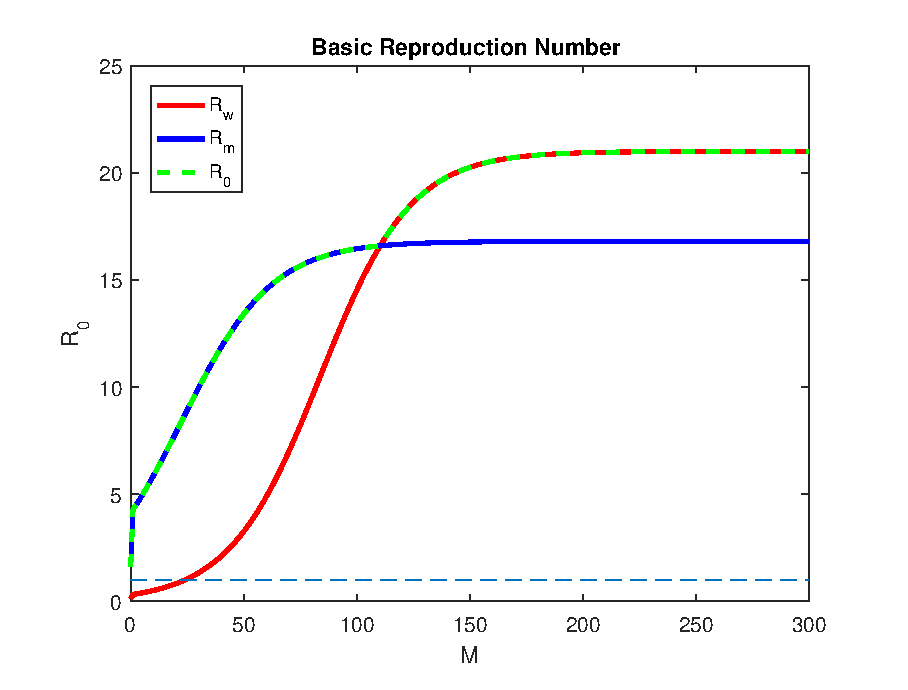
\includegraphics[scale=0.65]{brn.eps}
\caption{Computed values of $R_w$ and $R_m$ for increasing $M$. A population switch occurs at approximately $M=100$.}
\end{center}
\end{figure}


Setting $M=0$ results in $R_0 = R_m = 1.63$, indicating that the mutant virus is dominate when there is no morphine and that the IFE is unstable. A population switch occurs at approximately $M=100$ and the wild-type becomes dominant for any higher morphine concentrations. Note that $M=300$ results in $R_0 = R_w \approx 21$. In the next section, simulations of the steady state viral load will show that the dominance of the mutant virus contributes to the higher viral load when mophine is present.

\vspace{5mm}

 We now perform a sensitivity analysis to identify the paramters that have the greatest effect on the basic reporduction numbe \cite{Marino}. For a parameter $x$, the forward sensitivity index is given by \cite{Perera, Rodrigues}

\begin{center}
$\begin{array}{rcl}
S_x & = & \frac{x}{R_0}\frac{\partial R_0}{\partial x}
\end{array}$.
\end{center}

\vspace{5mm}

Using the parameter values in Table 1, the sensitivity indecies for $R_0^w$ and $R_0^m$ are given in the bar graphs below.

\begin{figure*}[h]
    \centering
    \begin{subfigure}[b]{0.5\textwidth}
        \centering
        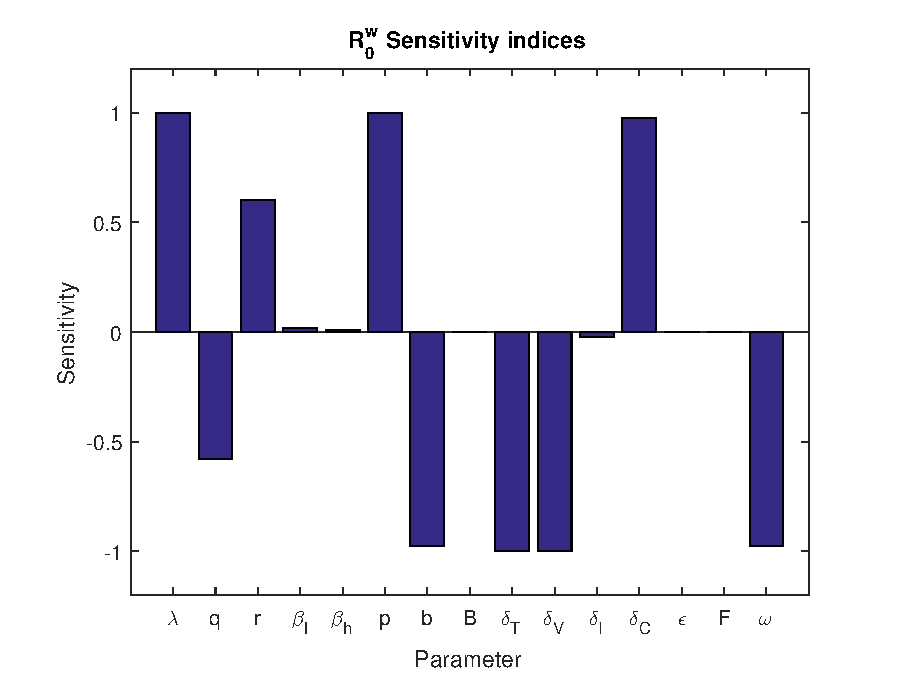
\includegraphics[scale=0.5]{Rw_sen.eps}
        %\caption{$R_w^0$ sensitivity indices}
    \end{subfigure}%
    ~ 
    \begin{subfigure}[b]{0.5\textwidth}
        \centering
        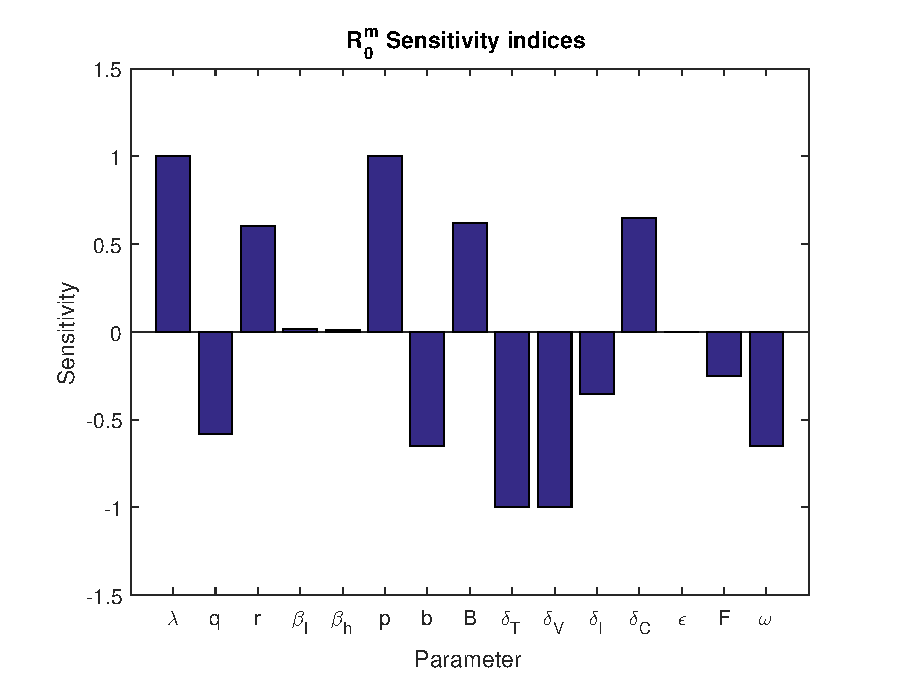
\includegraphics[scale=0.5]{Rm_sen.eps}
        %\caption{$R_w^0$ sensitivity indices}
    \end{subfigure}
    \caption{Sensistivity indices for $R_0^w$ and $R_0^m$}
\end{figure*}

%\begin{table}[H]
%\small
%\centering
%\caption{Sensitivity Indices, $M=300$}
%\begin{tabular}{|c||c|c|}
%\hline
  %& $R_0^w$ & $R_0^m$\\
%\hline
%$x$ & $S_x$ & $S_x$\\
%\hline
%$\lambda$ & $1$ & $1$\\
%\hline
%%$q$ & $0$ & $0$\\
%\hline
%$r$ & $0.018$ & $0.09$\\
%\hline
%$\beta_l$ & $0$ & $0$\\
%\hline
%$\beta_h$ & $0.99$ & $0.01$\\
%\hline
%$p$ & $1$ & $1$\\
%\hline
%$b$ & $-0.98$ & $-0.65$\\
%\hline
%$B$ & NA & $0.94$\\
%\hline
%$\delta_T$ & $-1.02$  & $-1.02$ \\
%\hline
%$\delta_V$ & $-1$ & $-1$ \\
%\hline 
%$\delta_I$ & $-0.025$ & $-0.35$\\
%\hline
%$\delta_C$ & $0.97$ & $0.65$\\
%\hline
%$\epsilon$ & $0$ & NA\\
%\hline
%$F$ & NA & $-0.25$\\
%\hline
%\end{tabular}
%\end{table}

%\begin{table}[H]
%\small
%\centering
%\caption{Sensitivity Indices, $M=0$}
%\begin{tabular}{|c||c|c|}
%\hline
  %& $R_0^w$ & $R_0^m$\\
%\hline
%$x$ & $S_x$ & $S_x$\\
%\hline
%$\lambda$ & $1$ & $1$\\
%\hline
%$q$ & $-0.58$ & $-0.58$\\
%\hline
%$r$ & $0.6$ & $0.6$\\
%\hline
%$\beta_l$ & $0.02$ & $0.02$\\
%\hline
%$\beta_h$ & $0.01$ & $0.01$\\
%\hline
%$p$ & $1$ & $1$\\
%\hline
%$b$ & $-0.98$ & $-0.65$\\
%\hline
%$B$ & NA & $0.92$\\
%\hline
%$\delta_T$ & $-1.02$  & $-1.02$ \\
%\hline
%$\delta_V$ & $-1$ & $-1$ \\
%\hline 
%$\delta_I$ & $-0.02$ & $-0.35$\\
%\hline
%$\delta_C$ & $1$ & $0.65$\\
%\hline
%$\epsilon$ & $0$ & NA\\
%\hline
%$F$ & NA & $-0.25$\\
%\hline
%\end{tabular}
%\end{table}

%\subsection{Dominant Viral Species}

%In order to observe the effect of morphine on $R_0$, and therefore on the viral load, $R_0^w$ and $R_0^m$ are calculated for various concentrations of morphine, noting that if $R_0^w > R_0^m$ the wild-type virus will be the dominate viral species while if $R_0^w < R_0^m$ the mutant will dominate. Using the Parameter values in Table 1 and letting $M$ vary from $0$ to $300$ gives the results shown Figure 1.

%\begin{figure}
%\centering
%\caption{Basic Reproduction Number}
%\includegraphics[scale=0.65]{basic_reproduction_number.eps}
%\caption{Computed values of $R_w$ and $R_m$ for increasing $M$. A population switch occurs at approximately $M=31$.}
%\end{figure}

%Setting $M=0$ results in $R_0 = R_m = 2.33$, indicating that the mutant virus is dominate when there is no morphine and that the IFE is unstable. A population switch occurs at approximately $M=100$ and the wild-type becomes dominant for any higher morphine concentrations. Note that $M=300$ results in $R_0 = R_w \approx 21$. In the next section, simulations of the steady state viral load will show that the dominance of the mutant virus contributes to the higher viral load when mophine is present.

\subsection{Stability Analysis}
\subsubsection{Mutant Only Equilibrium}

	%The mutant only equilibrium (MOE) is the equilibrium in which there is no wild-type virus present and is of the form $(T_l^*, T_h^*, 0, V_m^*, 0, I_m^*, C^*)$. Note that because of the mutation term in the equation for $I_m$ some mutant virus is being produced whenever the wild-type virus is present and for this reason there is no positive wild-type only equilibrium. The mutant only equilbrium is calculated by solving the system

%\begin{center}
%$\begin{array}{rcl}
 %0 & = &  \lambda + q T_h^* - r T_l^*  - \hat{\beta_l} V_m^* T_l^* - \delta_T T_l^* \\
%0 & = & r T_l^* - q T_h^*  - \hat{ \beta_h} V_m^* T_h^* - \delta_T T_h^* \\
%0 & = & p I_m^* - \delta_V V_m^*\\
%0 & = &\hat{\beta_l} V_m^* T_l^* + \hat{ \beta_h} V_m^* T_h^* -\frac{b}{1+B} I_m^* C^* -\delta_I I_m^*\\
%0 & = & \omega + \hat{\alpha} I_m^* C^* - \delta_C C^*\\
%\end{array}$
%\end{center}

The mutant only equilibrium is the equilibrium in which there is no wild-type virus present $(T_l^*, T_h^*,0,V_m^*,0,I_m^*,C^*)$, where

\begin{align*}
T_h^* & = \frac{r(M) \lambda}{(q(M) + \hat{\beta_h} V_m^* + \delta_T) ( r(M)+ \hat{\beta_l} V_m^* + \delta_T) -r(M)q(M)} \\
T_l^*  & = \frac{\lambda (q(M) + \hat{\beta_h} V_m^* +\delta_T)}{(q(M) + \hat{\beta_h} V_m^* + \delta_T) ( r(M)+ \hat{\beta_l} V_m^* + \delta_T) -r(M)q(M)} \\
%T_l^*  & =  \frac{r \lambda}{(q + \hat{\beta_h} V_m^* + \delta_T) ( r+ \hat{\beta_l} V_m^* + \delta_T) -rq}\cdot \frac{q + \hat{\beta_h} V_m^* +\delta_T}{r} \\
I_m^* & = \frac{\delta_V V_m^*}{p}\\
C^* & = \frac{\omega}{\delta_C - \hat{\alpha} \frac{\delta_V V_m^*}{p}} \\
\end{align*}

%\begin{center}
%$\begin{array}{rcl}
%T_h^* & = & \frac{\lambda}{(q + \hat{\beta_h}+\delta_T) \cdot [1 + \frac{\hat{\beta_l}  V_m^*}{r} +\frac{\delta_T}{r} - q]}\\
%T_l^* & = &  T_h^* \cdot \frac{q + \hat{\beta_h} V_m^* + \delta_T}{r}\\
 %I_m^* & = & \frac{\delta_V V_m^*}{p}\\
%C^* & = & \frac{\omega}{\delta_C - \hat{{\alpha}} I_m^*}\\
%\end{array}$
%\end{center}

%\vspace{5mm}

and $ V_m^*$ is the solution of

\begin{align*}
0 &= V_m^* \cdot g(V_m^*) \\%[\hat{\beta_l}T_h^* \cdot \frac{q+\hat{beta_h} V_m^*+\delta_T}{r}] + \hat{\beta_b} T_h^* - \frac{b}{1+B}(\frac{\delta_V}{p}(\frac{\omega}{\delta_C - \hat{\alpha}(\frac{\delta_V V_m^*}{p})) - \frac{\delta_I \delta_V}{p} \\
\end{align*}

where

\begin{align*}
g(V_m^*) & = \frac{\hat{\beta_l} \lambda \left(V_m^* \hat{\beta_h} + q(M) + \delta_T \right) + \hat{\beta_h} r \lambda   }   {\left(V_m^* \hat{\beta_h} + q(M) + \delta_T \right)  
  \left(V_m^* \hat{\beta_l} + r(M)+\delta_T \right) - r(M)q(M)} -  \frac{b \delta_V \omega}{ \left(1+B\right) p \left( \delta_C - \frac{\hat{\alpha} \delta_V V_m^*}{p}  \right)  }      
- \frac{\delta_I \delta_V}{p} . \\
\end{align*}

Clearly, $V_m^* = 0$ satisfies this equation, but this results in the IFE. The zeros of $g(V_m^*)$ can be found numerically and are plotted below for different values of $M$.

%\begin{center}
%$\begin{array}{rcl}
%0 & = & \hat{\beta_l} V_m^* [ \frac{r \lambda}{(q + \hat{\beta_h} V_m^* + \delta_T) ( r+ \hat{\beta_l} V_m^* + \delta_T) -rq} \cdot \frac{q + \hat{\beta_h} V_m^* + \delta_T}{r}] + \hat{\beta_h}V_m^*T_h^* \\
 %& &- \frac{b}{1+B}(\frac{\delta_V V_m^*}{p})(\frac{\omega}{\delta_C - \hat{\alpha}(\frac{\delta_V V_m}{p})}) - \frac{\delta_I %\delta_V V_m}{p}.\\
%\end{array}$
%\end{center}

%Substituting $T_h^*$ and solving numerically gives a value for $V_m^*$. Several values of $V_m^*$ are plotted in Figure 2 for different values of $M$.  Notably, increased values of $M$ cause an increase in $V_m^*$ and a decrease in $C^*$. For all values in Table 2, $F=0.2$ and $B=20.5$.

\begin{figure}[H]
\centering
%\caption{Solution of $V_m^*$ Equation}
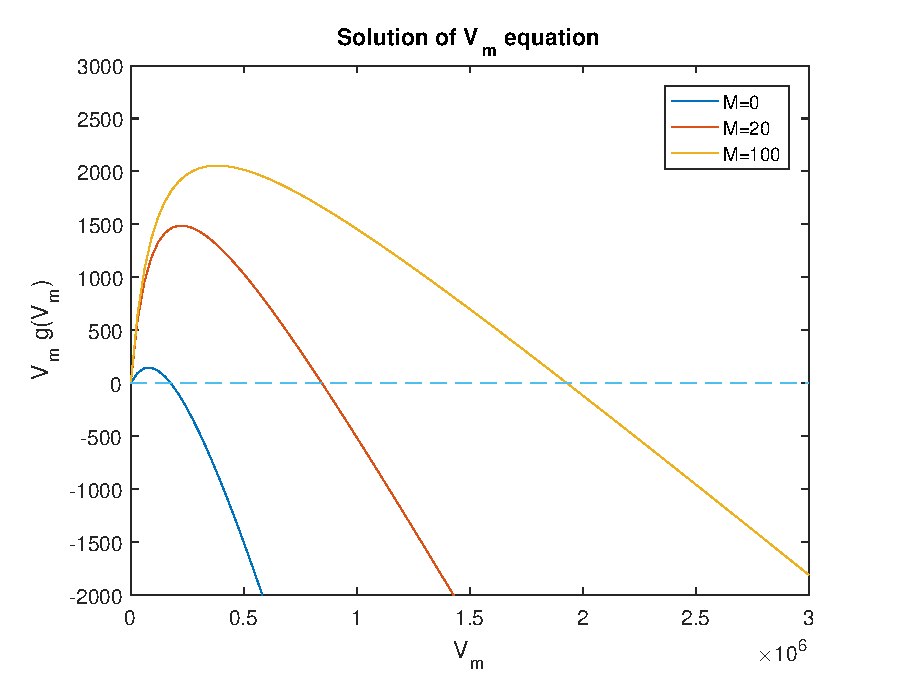
\includegraphics[scale=0.65]{V_m_sol.eps}
\caption{Solutions of $V_m^*$ equation. The zero-intercept of each curve is the MOE value of $V_m$ for the particular value of$M$.}
\end{figure}

%\begin{table}[H]
%\begin{table}[tbp]
%\centering
%\caption{Mutant Only Equilibrium}
%\begin{tabular}{|c|c|c|c|}
%\hline
%& $M=0$ & $M=20$ & $M=100$\\
%\hline
%$V_m$ & $3.93\times 10^5$ & $1.12\times 10^6$ & $1.95\times 10^6$\\
%\hline
%$T_h$ & $6.12\times 10^4$ & $3.62\times 10^4$ & $2.18\times 10^4$\\
%\hline
%$T_l$ & $1.12\times 10^5$ & $6.95\times 10^3$ & $6.94\times 10^3$\\
%\hline
%$I_m$ & $2.26\times 10^3$ & $6.46\times 10^3$ & $1.12\times 10^4$\\
%\hline
%$C$ & $81.32$ & $29.29$ & $0.54$\\
%\hline
%\end{tabular}
%\end{table}

To determine the stability of the MOE, we calculate the Jacobian matrix and evaluat it at the MOE. The Jacobian matrix is 

\vspace{5mm}

%\centering
\begin{center}
$\begin{array}{rcl}
J & = & \begin{bmatrix}
J_{11} & J_{12} & J_{13} & J_{14} & 0 & 0 & 0\\
J_{21} & J_{22} & J_{23} & J_{24} & 0 & 0 & 0\\
0 & 0 & J_{33} & 0 & J_{35} & 0 & 0\\
0 & 0 & 0 & J_{44} & 0 & J_{46} & 0 \\
J_{51} & J_{52} & J_{53} & 0 &J_{55} & 0 &J_{57}\\
J_{61} &J_{62} & J_{63} & J_{64} & 0 &J_{66} &  J_{67}\\
0 & 0 & 0 & 0 & J_{75} & J_{76} &J_{77}\\
\end{bmatrix}
\end{array}$
\end{center}

\vspace{5mm}

where

\vspace{5mm}

\begin{center}
%\centering
$\begin{array}{rclrcl}
J_{11} & =&-r - \beta_l V_w - \hat{\beta_l} V_m -\delta_T                  &J_{52} & = &(1 - \hat{\epsilon}) \beta_h V_w  \\
 J_{12} & = & q                            &J_{53} & = & (1 - \hat{\epsilon} )(\beta_l T_l + \beta_h T_h) \\
 J_{13} & = & -\beta_l T_l                            &J_{55} & = &  -bC - \delta_I  \\
 J_{14} & = &  -\hat{\beta_l} T_l                         &J_{57} & = &  -b I_w  \\
J_{21} & = & r                     & J_{61} & = &\hat{\epsilon}  \beta_l V_w + \hat{\beta_l} V_m \\
 J_{22} & = & -q-\beta_h V_w - \hat{\beta_h} V_m -\delta_T      & J_{62} & = &  \hat{\epsilon}  \beta_h V_w + \hat{\beta_h} V_m \\
J_{23} & = &  -\beta_h T_h                    & J_{63} & = & \hat{\epsilon} (\beta_l T_l + \beta_h T_h) \\%-\hat{\beta_h} T_h\\
 J_{24}& = &  -\hat{\beta_h} T_h                   & J_{64} & = &  \hat{\beta_l} T_l +\hat{\beta_h} T_h     \\
J_{33} & = &-\delta_V                   &J_{66} & = & -\frac{b}{1+B} C - \delta_I  \\
J_{35} & = & p                  &J_{67} & = &  -\frac{b}{1+B} I_m \\
 J_{44} & = & -\delta_V                &J_{75} & = & \hat{\alpha}  C  \\
 J_{46} &= & p            &J_{76} & = &  \hat{\alpha} C   \\
J_{51} & = & (1 - \hat{\epsilon}) \beta_l V_w               & J_{77} & = &  \hat{\alpha}(I_w + I_m) - C.   \\

 %J_{52} & = &(1 - \hat{\epsilon}) \beta_h V_w\\
%J_{53} & = & (1 - \hat{\epsilon} )(\beta_l T_l + \beta_h T_h)\\
%J_{55} & = &  -bC - \delta_I\\
%J_{57} & = &  -b I_w\\
%J_{61} & = &\hat{\epsilon}  \beta_l V_w + \hat{\beta_l} V_m\\
%J_{62} & = &  \hat{\epsilon}  \beta_h V_w + \hat{\beta_h} V_m\\
%J_{63} & = & \hat{\epsilon} (\beta_l T_l + \beta_h T_h)\\
% J_{64} & = &  \hat{\beta_l} T_l +\hat{\beta_h} T_h \\
%J_{66} & = & -\frac{b}{1+B} C - \delta_I \\
 %J_{67} & = &  -\frac{b}{1+B} I_m\\
% J_{75} & = & \hat{\alpha}  C \\
%J_{76} & = &  \hat{\alpha} C\\
%J_{77} & = &  \hat{\alpha}(I_w + I_m) - C.\\

\end{array}$
\end{center}

\vspace{5mm}

Note that the MOE is locally asymptotically stable if the real parts of each eigenvalue of $J$ is negative and unstable otherwise  \cite{Perko, Smith}. We now examine how the amount of morphine affects the stability of the MOE. We compute the maximum of the real parts of all eigenvalues of $J$ as a function of $M$, shown in Figure 4. Note that the real parts plotted in Figure 4 do not necessarily belong to the same eigenvalue. The MOE becomes unstable at $M \approx 110$, later we show that the wild-type virus dominates when $M$ exceeds this value.

% which can be done by plotting the real part of the maximum eigenvalue of $J$ as a function of $M$. Note that as $M$ varries different eigenvalues can have the maximal real part, and since the $max$ function is not differentiable everywhere, the function $max(\Re({\sigma(J)}))$ need not be differentiable everywhere.

\begin{figure}[H]
\centering
%\caption{Effect of $M$ on stability of MOE}
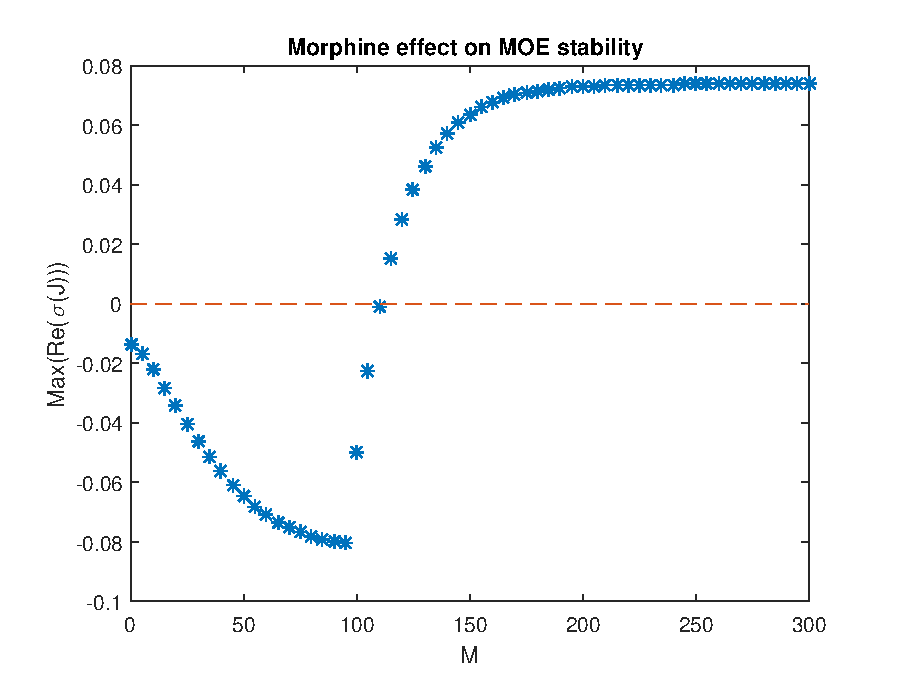
\includegraphics[scale=0.65]{MOE_morph.eps}
\caption{Effect of $M$ on the stability of the MOE. The MOE becomes unstable at approximately $M=110 ml/kg$.}
\end{figure}

The fitness cost $F$ and escape ratio $B$ also affect the stability of the MOE. The contour plot in Figure 5 shows the maximum real part of the eigenvalues of $J$ evaluated at the MOE as a function of both $F$ and $M$. Contours with a value less than 0 correspond to regions where the MOE is stable, and the figure shows that a low fitness cost can allow the mutant to dominate for higher concentrations of morphine. 

\begin{figure}[H]
\centering
%\caption{Effect of $M$ on stability of MOE}
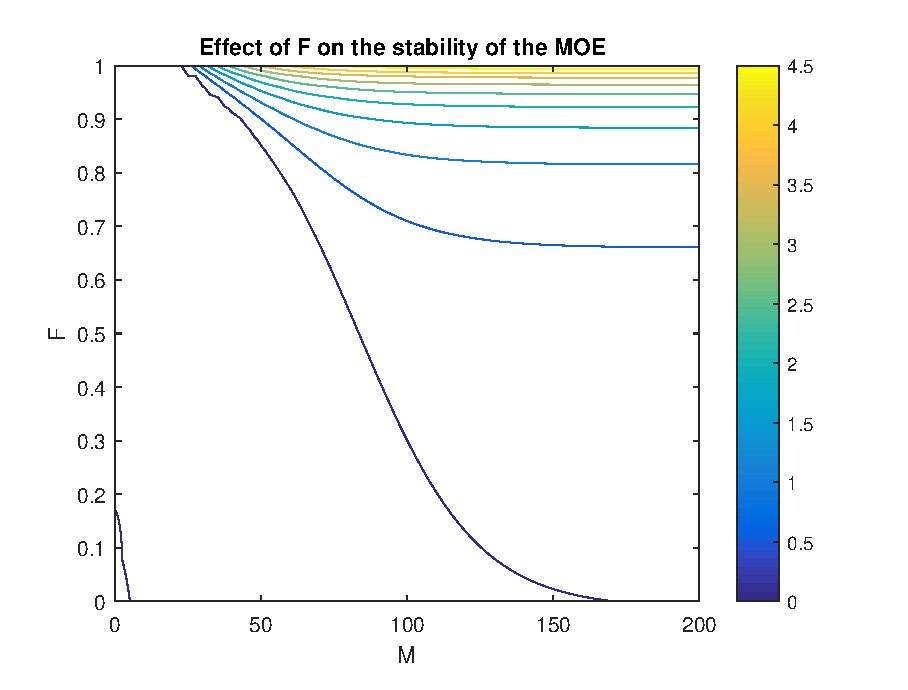
\includegraphics[scale=0.65]{F_M_cont.eps}
\caption{Effect of $F$ on the stability of the MOE}
\end{figure}

The contour plot in Figure 6 shows the maximum real part of the eigenvalues of $J$ evalueted at the MOE as a function of $B$ and $M$. Contours with a value less than 0 correspond to regions where the MOE is stable.

\begin{figure}[H]
\centering
%\caption{Effect of $M$ on stability of MOE}
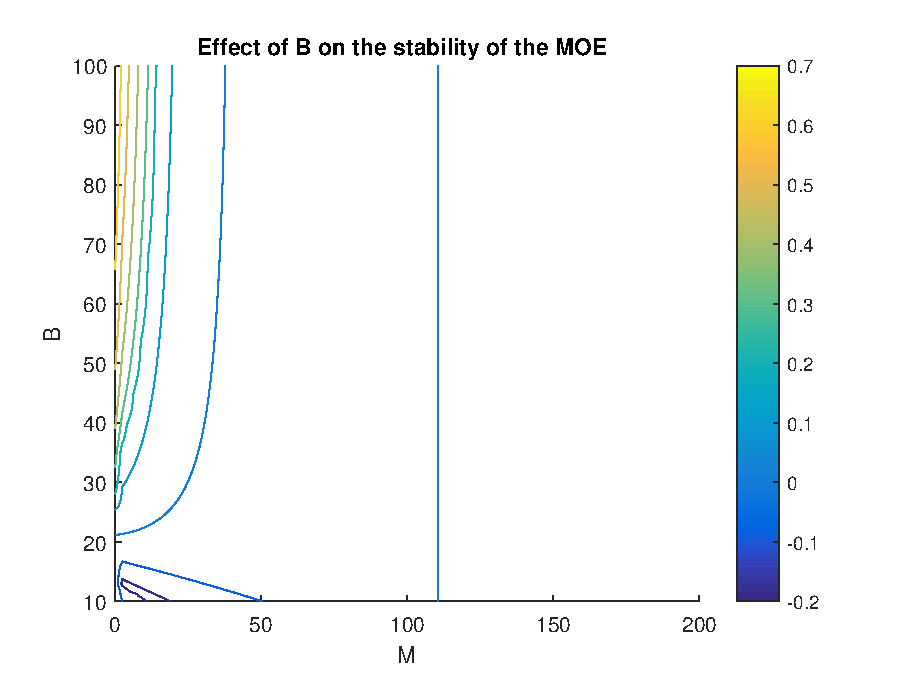
\includegraphics[scale=0.65]{B_M_cont.eps}
\caption{Effect of $B$ on the stability of the MOE}
\end{figure}


% Figure (?) shows $max(\Re({\sigma(J)}))$ as a function of $F$ for several values of $M$. Notably, as $M$ increases smaller values of $F$ result in the MOE becoming unstable. Similarly, increases in $M$ increase the value of $B$ which causes the MOE to become unstable.

%\begin{figure}[H]
%\centering
%\begin{subfigure}{.5\textwidth}
  %\centering
  %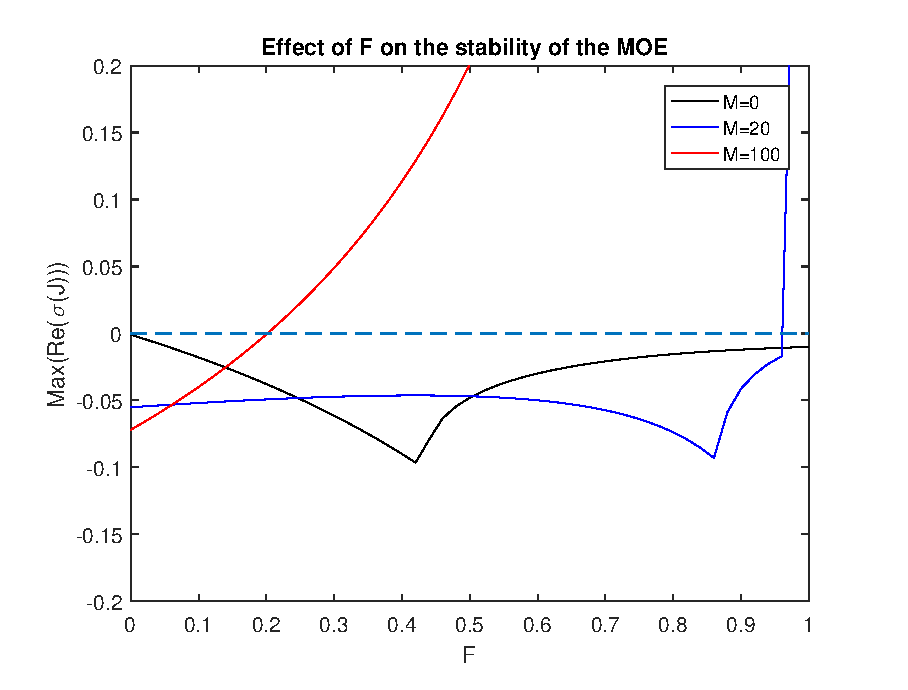
\includegraphics[scale = 0.5]{MOE_F.eps}
 % \caption{A subfigure}
 % \label{fig:sub1}
%\end{subfigure}%
%\begin{subfigure}{.5\textwidth}
  %\centering
  %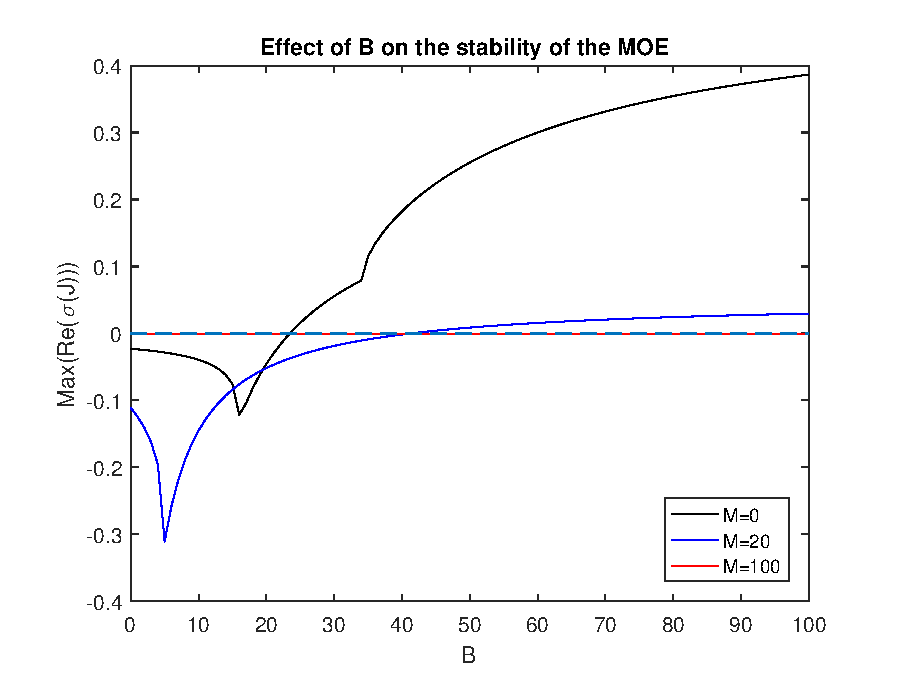
\includegraphics[scale = 0.5]{MOE_B.eps}
  %\caption{A subfigure}
% \label{fig:sub2}
%\end{subfigure}
%\caption{A figure with two subfigures}
%\label{fig:test}
%\end{figure}




%For $M=0$,

%\vspace{5mm}

%\begin{center}
%$\begin{array}{lcl}
%\sigma(J((T_l^*, T_h^*, 0, V_m^*, 0, I_m^*, C^*))) & = &   \{-23.3439, -0.0349\pm0.0894i, -0.5773,\\ %-0.4042, -23.3822, -0.4371\} \\
 %& & -0.4175, -23.4343, -0.2967\}\\
%\end{array}$
%\end{center}

%\vspace{5mm}

%and for $M=30$

%\vspace{5mm}

%\begin{center}
%$\begin{array}{lcl}
%\sigma(J((T_l^*, T_h^*, 0, V_m^*, 0, I_m^*, C^*))) & = &   \{-23.3099, -0.0351\pm0.0894i, -0.6281,\\ %-0.4042, -23.3822, -0.4371\} \\
% & & -0.4238, -23.3832, -0.0026\}\\
%\end{array}$
%\end{center}

%\vspace{5mm}

%so the MOE is  locally asymptotically stable for these values of $M$, but $M=300$ results in

%\vspace{5mm}

%\begin{center}
%$\begin{array}{lcl}
%\sigma(J((T_l^*, T_h^*, 0, V_m^*, 0, I_m^*, C^*))) & = &   \{-23.3010, -0.0357\pm0.0895i, -0.4255,\\ %-0.4042, -23.3822, -0.4371\} \\
 %& & -0.6298, -23.3738, 0.0738\}\\
%\end{array}$
%\end{center}

%\vspace{5mm}

%indicating the MOE becomes unstable by $M=300$. Assuming that the values of the MOE are constant around $M=30$ and taking the real part maximal eigenvalue of $J$ as a function of $M$ shows that a bifurcation takes place at $M \approx 31$ (Figure 3). It is also of interest to examine the effects of $F$ and $B$ on the stability of the MOE. Since the MOE is stable for $M= 30$, this is an acceptable value of $M$ to investigate the effects of $F$ and $B$. Figure 4 shows a bifurcation at approximately $F=0.21$ when $M=30$, identifying $F$ as a bifurcation parameter. However, Figure 5 shows that the real part of the maximal eigenvalue of $J$ is negative for any $B\in[1,100]$ at $M=30$, indicating that $B$ is not a bifurcation parameter for this amount of morphine.

%\begin{figure}
%\centering
%\caption{Effect of $M$ on stability of MOE}
%\includegraphics[scale=0.65]{MOE_M.eps}
%\caption{Effect of $M$ on the stability of the MOE. The MOE becomes unstable at approximately $M=31$.}
%\end{figure}

%\begin{figure}
%\centering
%\caption{Effect of $F$ on stability of MOE, $M = 30$. The MOE becomes unstable at approximately $F=0.21$.}
%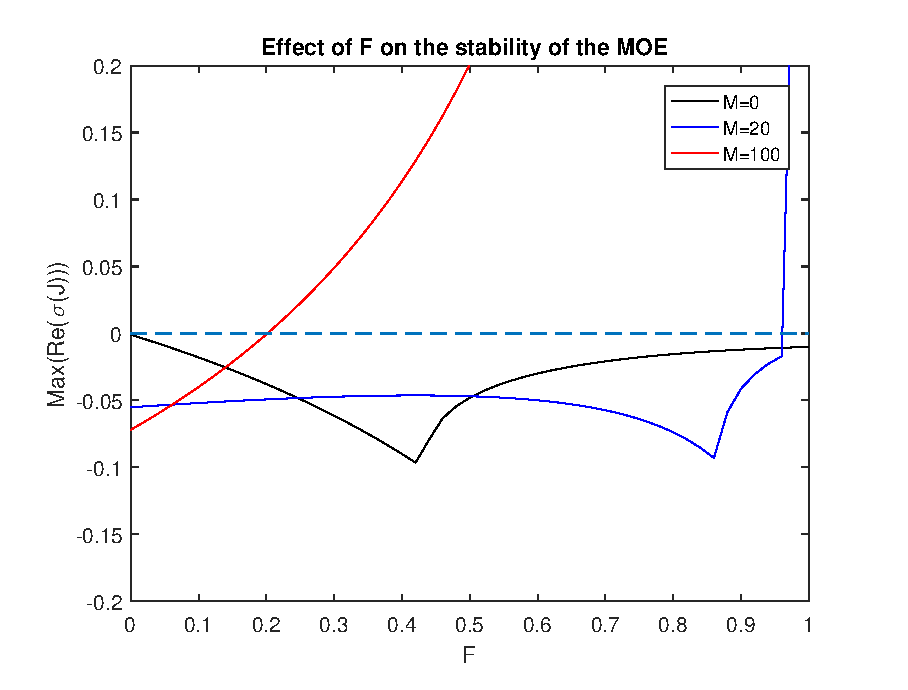
\includegraphics[scale=0.65]{MOE_F.eps}
%\caption{Effect of $F$ on the stability of the MOE, $M = 30$. The MOE becomes unstable at approximately $F=0.21$.}
%\end{figure}

%\begin{figure}
%\centering
%\caption{Effect of $B$ on stability of MOE, $M = 30$}
%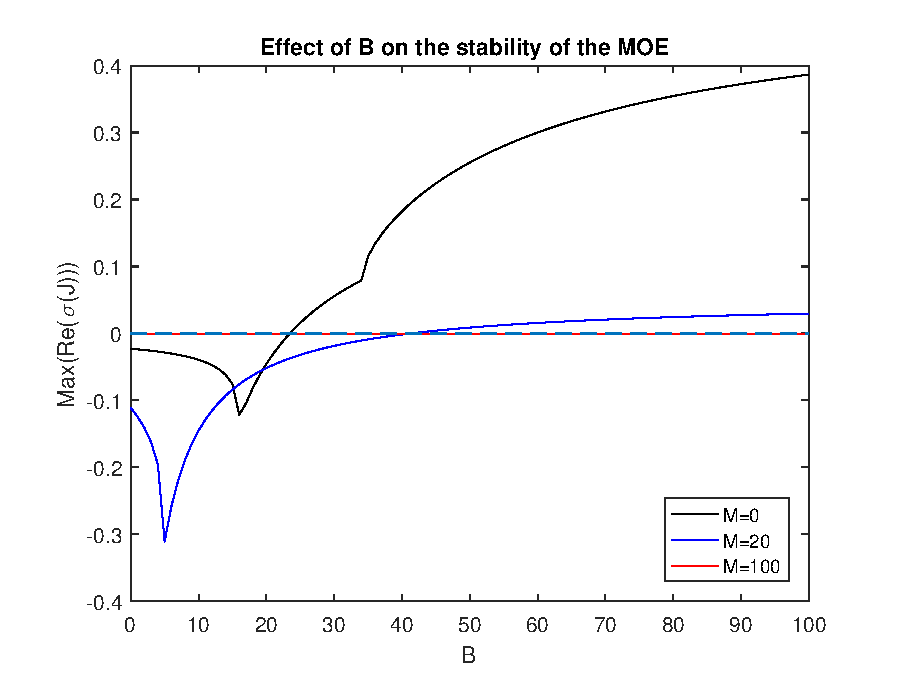
\includegraphics[scale=0.65]{MOE_B.eps}
%\caption{Effect of $B$ on the stability of the MOE, $M = 30$. The MOE remains stable for this range of $B$.}
%\end{figure}

\subsubsection{Wild-type Only Equilbirum}

A wild-type only equilibrium is a nonnegative solution of the form $(T_l^*, T_h^*, V_w^*,$
$ 0,  I_w^*, 0, C^*)$ to the system of equations 

\vspace{5mm}

\begin{center}
$\begin{array}{rcl}
 0 & = &  \lambda + q T_h - r T_l  - {\beta_l} V_w T_l - \delta_T T_l \\
0 & = & r T_l - q T_h  -  \beta_h V_w T_h - \delta_T T_h\\
0 & = & p I_w - \delta_V V_w\\
0 & = & (1-\hat{\epsilon})(\beta_l V_w T_l + \beta_h V_w T_h) - b I_w C - \delta_I I_w\\
0 & = & \hat{\epsilon}(\beta_l V_w T_l + \beta_h V_w T_h) \\
0 & = & \omega + \hat{\alpha} I_w C - \delta_C C.\\
\end{array}$
\end{center}

\vspace{5mm}

Solving the second equation for $T_h^*$ gives:

\vspace{5mm}

\begin{center}
$\begin{array}{rcl}
 T_h^* & = &  \frac{r}{q+\beta_h V_w^*  + \delta_T} T_l^*\\
\end{array}$
\end{center}

\vspace{5mm}

and the fifth equation is equivalent to (since $\epsilon \neq 0$)

\vspace{5mm}

\begin{center}
$\begin{array}{rcl}
 0 & = & \beta_l V_w T_l + \beta_h V_w T_h.\\
\end{array}$
\end{center}

\vspace{5mm}

If $V_w^* = 0$ this system is exactly the IFE, so cancelling $V_w^*$ and substituting $T_h^*$ gives:

\vspace{5mm}

\begin{center}
$\begin{array}{rcl}
 0 & = &  T_l^* ( \beta_l + \beta_h ( \frac{r}{q+\beta_h V_w^*  + \delta_T} ))\\
\end{array}$
\end{center}

\vspace{5mm}

so either  $T_l^* = 0$ or $\beta_l + \beta_h ( \frac{r}{q+\beta_h V_w^*  + \delta_T})  = 0$. Substituting $T_l^* = 0$ into the first equation results in the negative solution $T_h^* = -\frac{\lambda}{q}$. Letting $\beta_l + \beta_h ( \frac{r}{q+\beta_h V_w^*  + \delta_T})  = 0$ is equivalent to 

\vspace{5mm}

\begin{center}
$\begin{array}{rcl}
 V_w^* & = & -\frac{1}{\beta_h}(\frac{\beta_h r}{\beta_l} + q + \delta_T)     \\
\end{array}$
\end{center}

\vspace{5mm}

which is also a negative solution, and there is no nonnegative wild-type only equilibrium.

\subsection{Long-term Viral Dynamics}

Using the initial values and parameters given in Section 2.2 along with $F=0.2$, $B=20.5$, $\psi = 0.05$ and $\mu = \eta = \gamma = \xi = 1$ the model is solved using the ode15s function in MATLAB over a period of $100$ days. 

\begin{figure}[H]
\centering
%\caption{Total Viral Load (Base case)}
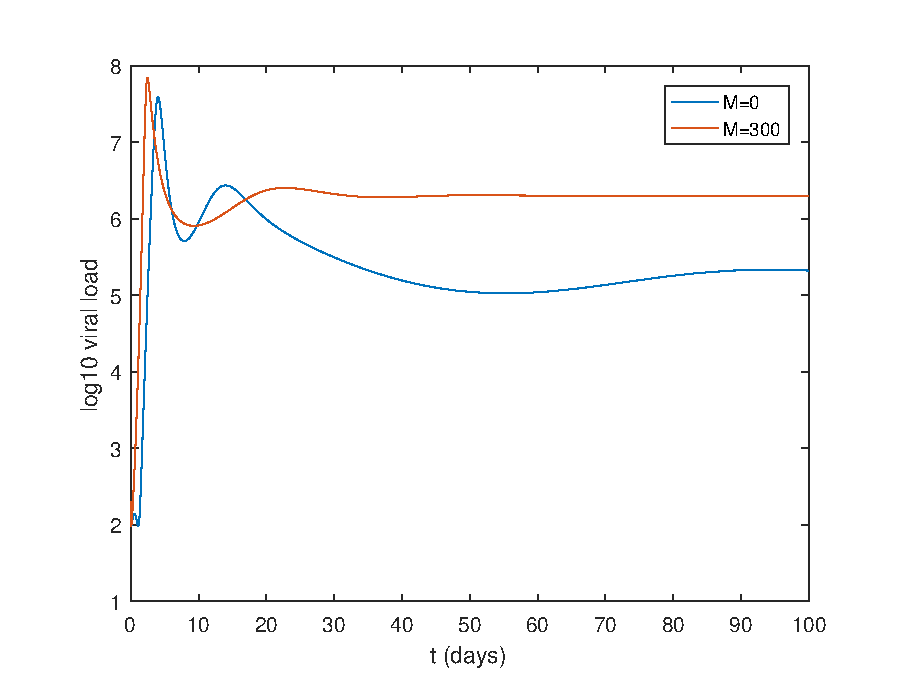
\includegraphics[scale=0.5]{viral_load_base.eps}
\caption{Total viral load with base parameter values. The model reflects the higher viral load caused by morphine.}
\end{figure}

Both cases show a rapid inintial increase in viral load, but the presence of morphine causes a higher peak viral load and steady state than the control simulation. Analysis of the basic reproduction number showed that a population switch occurs at approximately $M=100ml/kg$, so it is of interest to observe how the individual viral populations behave for values of $M$ above and below the threshold value. With $M=0$, the wild-type viral load quickly declines to zero and the total viral load in entirely mutant virus. With $M=150$, the wild-type virus is the dominant spices but due to mutation there is a small amount of mutant virus being continuously produced. These simulations are consistent with the analysis of the basic reproduction number and its dependence on $M$.

\begin{figure}[H]
\centering
\begin{subfigure}{.5\textwidth}
  \centering
  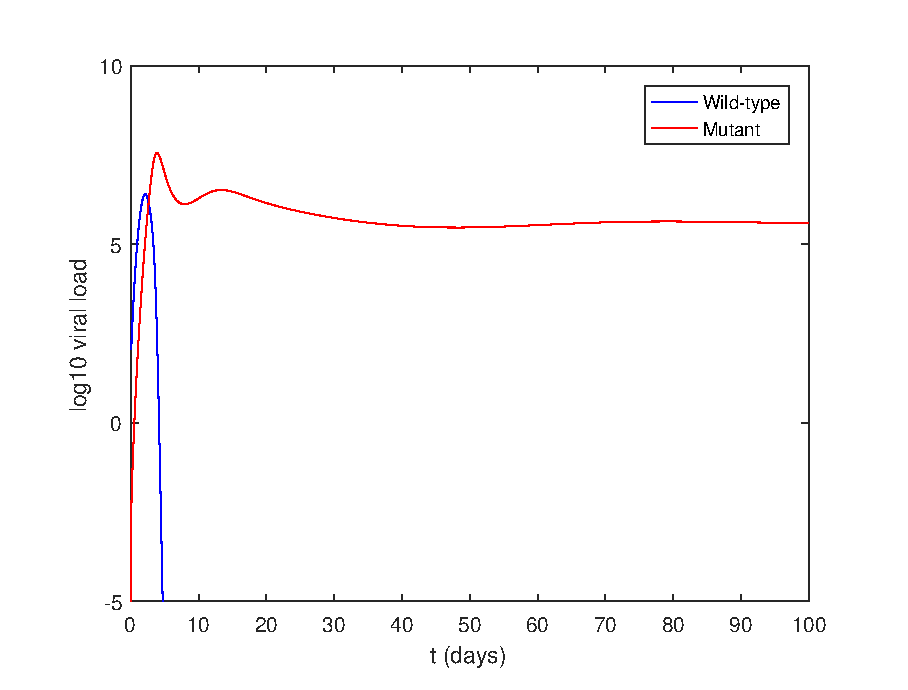
\includegraphics[scale = 0.5]{control_dynamics.eps}
  \caption{Individual viral populations, $M=0$}
 % \label{fig:sub1}
\end{subfigure}%
\begin{subfigure}{.5\textwidth}
  \centering
  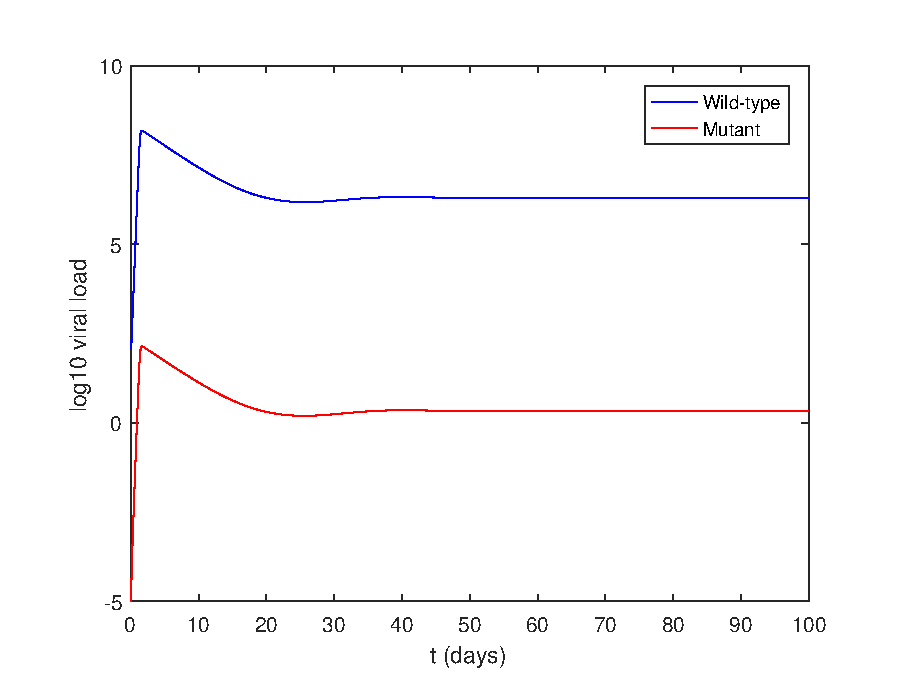
\includegraphics[scale = 0.5]{morphine_dynamics.eps}
  \caption{Individual viral populations, $M=150$}
% \label{fig:sub2}
\end{subfigure}
%\caption{A figure with two subfigures}
\label{fig:test}
\end{figure}



%Whether or not morphine is present, the viral load rapidly increases to approximately $7.5$ log10 before decreasing to a steady state of approximately $5.9$ log10 for $M=0$ and $6$ log10 for $M=300$ with a difference in viral load of approximately $2.18840 \times 10^5$ between the two cases (Figure 6). Decreasing $B$ from $10$ to $1$ (Figure 7) increase the difference in the steady state viral load to $7.27520 \times 10^5$, which is closer to results obtained experimentaly \cite{Kumar}.

%\begin{figure}
%\
%\caption{Total Viral Load (Decreased escape ratio)}
%\includegraphics[scale=0.65]{viral_load_decreased_b.eps}
%\caption{Total viral load with decreased escape ratio. Decreasing the escape ratio gives a differnce in viral load closer to experimental results. }
%\end{figure}



	%As discussed in Section 3.2, a population switch occurs at $M \approx 31$ for the base parameter values. Therefore, it is of interest to observe the populations of the individual species in the cases where the wild-type dominates and in the case where the mutant dominates. Figure 8 separately shows the populations of the wild-type and mutant when $M=0$. In this case, the logarithm of the wild-type virus becomes negative indicating that the wild-type population is approaching zero and the total viral load is essentially only the mutant population.

%\begin{figure}
%\centering
%\caption{Wild- type Population, $M=0$}
%\includegraphics[scale=0.65]{Mequalzero.eps}
%\caption{Individual virus populations, $M=0$. When no morphine is present the mutant is the dominant species.}
%\end{figure}



% Figure 9 shows the individual populations for $M=300$, a high enough morphine concentration for the wild-type to dominate. In this case the wild-type makes up the bulk of the viral load, however, due to mutation a small amount of mutant virus continues to be produced. These simulations are in agreement with the population switch discussed in Chapter 4.



%\begin{figure}
%\centering
%\caption{Wild- type Population, $M=0$}
%\includegraphics[scale=0.65]{Mequal300.eps}
%\caption{Individual virus populations, $M=300$. For this amount of morphine the wild-type is the dominant species.}
%\end{figure}

%\begin{figure}
%\centering
%\caption{Steady State Viral Load}
%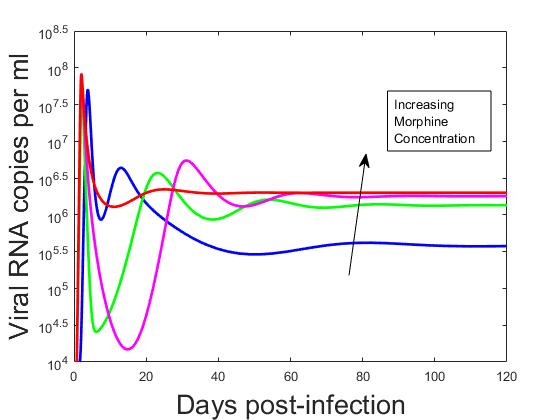
\includegraphics[scale=0.65]{dose.eps}
%\caption{Viral load at 200 days as a function of $M$.  }
%\end{figure}



%Figure 10 shows the effect on the viral load at 200 days as a function of the morphine concentration. There is a roughly $0.5$ log10 difference in viral load between the $M=0$ and $M=300$ cases and the viral load is most sensetive to changes in $M$ when $0<M<50$.



\section{Discussion}

We present a mathematical model to describe the within-host viral dynamics of an HIV infection which considers escape mutants, the use of morphine, and different populations of target cells based on susceptibility to infection. The model is primarily based on earlier models from \cite{Vaidya, Konrad} and simulates the increase in viral load that results from the use of morphine by introducing terms that lower the mutation rate of the virus and host's cellular immune response. Values of parameters in the model where taken both from earlier studies that provided estimates and from experimental data. 

	The basic reproduction number of each viral spiecies is calculated by way of the next-generation matrix method. The basic reproduction number was taken as a function of the concentration of morphine present and it was observed that a population switch occurs for a sufficiently high morphine concentration. At higher concentrations of morphine the wild-type virus dominates the mutant, but the reduced cellular immune response still results in a higher set point viral load. The infection free equilibrium is unstable regardless of whether or not morphine is present. The mutant only equilibrium is also stable for a sufficiently low morphine concentration and fitness cost of the virus, but becomes unstable as these parameters increase.

	Short- and long-term viral dynamics are simulated by solving the model numerically. If there is sufficient morphine for the wild-type virus to dominate a small amount of the mutant will persist due to mutation. If the mutant is the dominant species then it will effectively make up the entirety of the viral load. Varying the morphine concentration causes changes in the set point viral load for low concentrations, but the viral load stabilizes once the morphine concentration exceeds approximately $100 ml/kg$. 
	
	One limitation of the model is the assumption that the morphine concentration $M$ is constant with respect to time. This assumption is made for simplicity in calculations and for providing an easy way to determine the morphine concentration neccessary for the population switch to occur. Future work will focus on developing a method to incorporate a time-dependent morphine concentration and determining how this would affect the dynamics. It will also be of interest to investigate the sensitivity of the parameters introduced to model morphine effects, namely $\mu, \eta,\gamma$ and $\xi$, establish for them, and determining their effect on the stability of the equilbria of the model. Additionally, since it is possible for both the infection free and mutant only equilibria to be unstable it will be important to investigate any scenarios in which the wild-type and mutant coexist.  


\begin{thebibliography}{99}
\itemsep 0pt\relax

\bibitem{MMWR}
{\em Morbidity and motality weekly report}. vol. 59 (2010) pp. 1550-1555.
%Morbidity and Mortality Weekly Report. Vol 59, No 47 (December 3, 2010), pp 1550-1555

\bibitem{Kumar}
R. Kumar, C. Torres, Y. Yamamura, I. Rodriguez, M. Martinez, S. Staprans, R. M. Donahoe, E. Kraiselburd, E. B. Stephens, and A. Kumar,  {\em Modulation by morphine of viral set point in rhesus macaques infected with simian immunodeficiency virus and simian-human immunodeficiency virus}, J. Virol. vol. 78 (2004) pp. 11425-11428.
%Kumar, R., Torres, C., Yamamura, Y., Rodriguez, I., Martinez, M., Staprans, S., Donahoe, R. M., Kraiselburd, E., Stephens, E. B., and Kumar, A. {\em Modulation by Morphine of Viral Set Point in Rhesus Macaques Infected with Simian Immunodeficiency Virus and Simian-Human Immunodeficiency Virus}, Journal of Virology, Oct 2004 p. 11425-11428.

\bibitem{Hauser}
K. F. Hauser, Y. K. Hahn, V. V. Adjan, S. Zou, S. K. Buch, A. Nath, A. J. Bruce-Kelle, and P. E. Knapp, {\em HIV-1 tat and morphine have interactive effects on oligodendrocyte survival and morphology},  Glia vol.  57 (2009) pp. 194-206. doi:10.1002/glia.20746.
%Hauser, K. F., Hahn, Y. K., Adjan, V. V., Zou, S., Buch, S. K., Nath, A., Bruce-Kelle, A. J., Knapp, P. E. {\em HIV-1 Tat and Morphine Have Interactive Effects on Oligodendrocyte Survival and Morphology}. GLIA 57:194-206 (2009).

\bibitem{Greenough}
T. C. Greenough, D. B. Brettler, M. Somasundaran, D. L. Panicali and J. L. Sullivan,  {\em Human immunodeficiency virus type 1- specific cytotoxic T lymphocytes (CTL), virus load, and CD4 T cell loss: evidence supporting a protective role for CTL in vivo}, J. Infect. Dis. vol. 176 (1997) pp. 118-125.
%Greenough, T. C., Brettler, D. B., Somasundaran, M., Panicali, D. L., Sullivan, J. L. {\em Human Immunodeficiency Virus Type 1- Specific Cytotoxic T Lymphocytes (CTL), Virus Load, and CD4 T Cell Loss: Evidence supporting a Protective Role for CTL in vivo}. The Journal of Infectious Diseases, Vol. 176, No 1 (Jul., 1997), pp 118-125.

\bibitem{Boutwell}
C. L. Boutwell, M. M. Rolland, J. T. Herbeck, J. I. Mullins, and T. M. Allen,  {\em Viral evolutions and escape during acute HIV-1 infection}, J. Infect. Dis. vol. 202 (2010) pp. S309-S314.
%Boutwell, C. L., Rolland, M. M., Herbeck, J. T., Mullins, J. I., Allen, T. M. {\em Viral Evolutions and Escape during Acute HIV-1 Infection}. The Journal of Infectious Diseases, Vol. 202, Supplement 2. Primary HIV-1 Infection (15 October 2010), pp. S309-S314.

\bibitem{Perelson}
A. S. Perelson and  R. M. Ribeiro, {\em Modeling the within-host dynamics of HIV infection}, BMC Biol. (2013) http://www.biomedcentral.com/1741-7007/11/96
%Perelson, A. S., Ribeiro, R. M.{\em Modeling the within-host dynamics of HIV infection}. BMC biology. 2013;11:96. pmid:24020860; PubMed Central PMCID: PMC3765939.

\bibitem{Chubb}
M. C. Chubb and K. H. Jacobsen,  {\em Mathematical modeling and the epidemiological research process}, Eur. J. Epidemiol. vol. 25 (2010) pp. 13-19.
%Chubb, M. C., Jacobsen, K. H. {\em Mathematical Modeling and the Epidemiological Research Process}. European Journal of Epidemiology. Vol. 25, No. 1 (2010), pp. 13-19.

\bibitem{Kitchen}
S. G. Kitchen, J. K. Whitmire, N. R. Jones, Z. Galic, C. M. R. Kitchen, R. Ahmed, J. A. Zack, and F. V. Chisari,  {\em The CD4 molecule on CD8+ T lymphocytes directly enhances the immune response to viral and cellular anitgens}, Proc. Natl. Acad. Sci. U.S.A. vol. 102 (2005) pp. 3794-3799.
%Kitchen, S. G., Whitmire, J. K., Jones, N. R., Galic, Z., Kitchen, C. M. R., Ahmed, R., Zack, J. A., Chisari, F. V. {\em The CD4 Molecule on CD8+ T Lymphocytes Directly Enhances the Immune Response to Viral and Cellular Anitgens}. Proceedings of the National Academy of Sciences of the United States of America, Vol. 102, No. 10 (Mar., 8, 2005), pp. 3794-3799.

\bibitem{Killeen}
N. Kileen, C. B. Davis, K. Chu, M. E. C. Crooks, S. Sawada, J. D. Scarborough, K. A. Boyd, S. G. Stuart, H. Xu, and D. R. Littman, {\em CD4 function in thymocyte differentiation and T cell activation}, Philos. Trans. R. Soc. Lond., B, Biol. Sci. vol. 342 (1993) pp. 25-34.
%Killeen, N., Davis, C. B., Chu, K., Crooks, M. E. C., Sawada, S., Scarborough, J. D., Boyd, K. A., Stuart, S. G., Xu, H, Littman, D. R. {\em CD4 Function in Thymocyte Differentiation and T Cell Activation}. Philosophical Transaction: Biological Sciences, Vol. 342, No, 1299, The CD4 Lymphocyte Glycoprotein in Health and Disease (Oct. 29, 1993), pp. 25-34.

\bibitem{Chan}
D. C. Chan and P. S. Kim, {\em HIV entry and its inhibition}, Cell. vol. 93 (1998) pp. 681-684.
%Chan, D. C., Kim, P. S. {\em HIV Entry and Its Inhibition}. Cell, Vol. 93, 681-684, May 29, 1998.

\bibitem{Fauci}
A. S. Fauci, {\em Pathogensis of HIV disease: Opportunities for new prevention interventions}, Clin. Infect. Dis. vol. 45 (2007) pp. S206-S212.
%Fauci, A. S. {\em Pathogensis of HIV Disease: Opportunities for New Prevention Interventions}. Clinical Infections Diseases, Vol 45, Supplement 4. Opportunites for Improving the Diagnosis of Prevention of and Access to Treatment for HIV Infection in the United States (Dec. 15, 2007), pp. S206-S212.

\bibitem{McMichael}
A. J. McMichael and S. L. Rowland-Jones, {\em Cellular immune responses to HIV}, Nature vol. 410 (2001) pp. 980-987.
%McMichael, A. J., Rowland-Jones, S. L. {\em Cellular immune responses to HIV}. Nature, Vol. 410, 19 April, 2001.

\bibitem{Deng}
L. Deng, M. Pertea, A. Rongvauz, L. Want, C. M. Durand, G. Ghiaur, J. Lai, H. L. McHugh, H. Hao, J. B. Margolick, C. Gurer, A. J. Murphy, D. M. Valenzuela, G. D. Yancopoulus, S. G. Deeks, T. Stowig, P. Kumar, J. D. Siliciano, S. L. Salzberg, R. A. Flavell, L. Shan, and R. F. Siliciano, {\em Broad CTL response is required to clear latent HIV-1 due to dominance of escape mutations}, Nature vol. 517 (2015) pp. 381-385.
%Deng, L., Pertea, M., Rongvaux, A., Wang, L., Durand, C. M., Ghiaur, G., Lai, J., McHugh, H. L., Hao, H., Margolick, J. B., Gurer, C., Murphy, A.J., Valenzuela, D. M., Yancopoulos, G. D., Deeks, S. G., Strowig, T., Kumar, Priti., Siliciano, J. D., Salzberg, S. L., Flavell, R. A., Shan, L., Siliciano, R. F. {\em Broad CTL response is required to clear latent HIV-1 due to dominance of escape mutations}. Nature, Vol. 517, 15 January, 2015.

\bibitem{Ribeiro}
R. M. Ribeiro, L. L. Chavez, D. Li, S. G. Self, and A. S. Perelson, {\em Estimation of the initial viral growth rate and basic reproductive number during acute HIV-1 infection}, J. Virol. vol. 84 (2010) pp. 6096-6102.
%Ribeiro, R. M., Chavez, L. L., Li, D., Self, S. G., Perelson, A. S. {\em Estimation of the Initial Viral Growth Rate and Basic Reproductive Number during Acute HIV-1 Infection}. Journal of Virology, June 2010, p. 6096-2102.


\bibitem{Ganusov}
V. V. Ganusov, R. A. Neher, and A. S. Perelson, {\em Mathematical modeling of escape of HIV from cytotoxic T lymphocyte responses}, J. Stat. Mech. P01010-.foi:10.1088/1742-5468/2013/01/P01010.

\bibitem{Li}
Y. Li, X. Wang, S. Tian, C. Guo, S. D. Douglas, and W. Ho, {\em Methadone enhances human immunodeficiency virus infection of human immune cells}, J. Infect. Dis. vol. 185 (2002) pp. 118-122.
%Li, Y., Wang, X., Tian, S., Guo, C., Douglas, S. D., Ho, W. {\em Methadone Enhances Human Immunodeficiency Virus Infection of Human Immune Cells}. The Journal of Infectious Diseases, Vol. 185, No. 1 (Jan. 1, 2002). pp 118-122.

\bibitem{Noel1}
R. Noel, Z. Marrero-Otero, R. Kumar, G. S. Chompre-Gonzalez, A. S. Verma, and A, Kumar,  {\em Correlation between SIV tat evolution and AIDS progression in cerebrospinal fluid of morphine-dependent and control macaques infected with SIV and SHIV}, Virology vol. 349 (2006) pp. 440-452.
%Noel, R., Marrero-Otero, Z., Kumar, R., Chompre-Gonzalez, G.S., Verma, A.S., Kumar, A. (2006). {\em Correlation between SIV Tat evolution and AIDS progression in cerebrospinal fluid of morphine-dependent and control macaques infected with SIV and SHIV}. Virology 349(2):440-52. Epub 2006 Apr 27.

\bibitem{Noel2}
R. Noel and A. Kumar, {\em SIV vpr evolution is inversely related to disease progression in a morphine-dependent rhesus macaque model of AIDS}, Virology vol. 359 (2007) pp. 397-404.
%Noel, R., Kumar, A. (2007). {\em SIV Vpr evolution is inversely related to disease progression in a morphine-dependent rhesus macaque model of AIDS.} Virology 359-404.

\bibitem{Rivera-Amill}
V. Rivera-Amill, P. S. Silverstein, R. Noel, S. Kumar, and A. Kumar,  {\em Morphine and rapid disease progression in nonhuman primate model of AIDS: Inverse correlation between disease progression and virus evolution}, J. Neuroimmune Pharmacol vol. 5 (2014) pp. 122-132. http://doi.org/10.1007/s11481-009-9184-0
%Rivera-Amill, V., Silverstein, P.S., Noel, R., Kumar, S., Kumar, A. (2010). {\em Morphine and Rapid Disease Progression in Nonhuman Primate Model of AIDS: Inverse Correlation between Disease Progression and Virus Evolution.} J Neuroimmune Pharmacol (2010) 5:122-132.

\bibitem{Konrad}
B. P. Konrad, N. K. Vaiyda, and R. J. Smith?, {\em Modeling mutation to a cytotoxic T-lymphocyte HIV vaccine}, Math. Popul. Stud. vol. 18 (2011) pp. 122-149.
%Konrad, B. P., Vaidya, N. K., Smith?, R. J. (2008). {\em Modeling Mutation to a Cytotoxic T-lymphocyte HIV Vaccine} Mathematical Population Studies 18:122-149.

\bibitem{Schwartz}
E. S. Schwartz, K. R. H. Biggs, C. Bailes, K. A. Ferolito, and N. K. Vaidya, {\em HIV dynamics with immune responses: Perspectives from mathematical modeling}, Curr. Clin. Microbiol. Rep. vol. 3 (2016) pp. 216-224.
%Schwartz, E. S., Biggs, K. R. H., Bailes, C., Ferolito, K. A., Vaidya, N. K., (2016) {\em HIV Dynamics With Immune Responses: Perspectives From Mathematical Modeling} Virology DOI 10.1007/s40588-016-0049-z.

\bibitem{Vaidya}
N. K. Vaidya, R. M. Ribeiro, A. S. Perelson, and A. Kumar,  {\em Modeling the effects of morphine on simian immunodeficiency virus dynamics}, PloS Comput. Biol. (2016) https://doi.org/10.1371/journal.pcbi.1005127
%Vaidya N. K., Ribeiro R. M., Perelson A. S., Kumar A. (2016). {\em Modeling the Effects of Morphine on Simian Immunodeficiency Virus Dynamics.} PLoS Comput Biol 12(9): e1005127. https://doi.org/10.1371/journal.pcbi.1005127.

\bibitem{Castillo-Chavez}
C. Castillo-Chavez, Z. Feng, and W. Huang,  {\em On the computation of $R_0$ and its role on global stability}, Mathematical Approaches for Emerging and Reemergin Infections Diseases: An Introduction, Springer-Verlag, New York, 2002, pp. 229-250.
%C. Castillo-Chavez, Z. Feng and W. Huang, “On the Computation of R0 and Its Role on Global Stability,” In: Mathematical Approaches for Emerging and Reemerging Infectious Diseases: An Introduction, Springer-Verlag, New York, 2002, pp. 229-250. doi:10.1007/978-1-4613-0065-6

%Castillo-Chavez, C., Feng, Z., Huang, W. {\em On the Computation of $R_0$ and its Role on Global Stability}, (2001).

\bibitem{Olkkola}
K. T. Olkkola, E. Maunuksela, R. Korpela, and P. H. Rosenberg,  {\em Kinetics and dynamics of postperative intravenous morphine in children}, Clin. Pharmacol. Ther. vol. 44 (1988) pp. 128-136.
%Olkkola, K. T., Maunuksela, E., Korpela, R., Rosenberg, P. H. {\em Kinetics and dynamics of postperative intravenous morphine in children.} (1988).

\bibitem{Perko}
L. Perko, {\em Differential equations and dynamical systems}, 2nd ed., Springer-Verlag, New York, 1991.
%Perko, L. {\em Differential Equations and Dynamical Systems}. Springer-Verlag, New York, NY, (1991).

\bibitem{Jordan}
D. W. Jordan and P. Smith,  {\em Nonlinear ordinary differential equations: An introduction to dynamical systems}, 3rd ed. Oxford University Press, New York, 1999.
%Jordan, D. W., Smith, P. {\em Nonlinear Ordinary Differential Equations: An Introduction to Dynamical Systems}. Oxford University Press, New York, NY, (1999).

\bibitem{Ganusov}
V. V. Ganusov and R. J. De Boer, {\em Estimating costs and benefits of CTL escape mutations in SIV/HIV infection}, PloS Comput. Biol.(2006) https://doi.org/10.1371/journal.pcbi.0020024
%Ganusov, V.V., De Boer, R. J. {\em Estimating Costs and Benefits of CTL Escape Mutations in SIV/HIV Infection}. Plos Comput Biol 2(3): e24 (2006).

\bibitem{Smith}
R. J. Smith and L. M. Wahl,  {\em Drug resistance in an immunological model of HIV-1 infection with impulsive drug effects}, Bull. Math. Biol. vol. 67 (2005) pp. 783-813.
%Smith, R. J., Wahl, L. M. {\em Drug resistance in an immunological model of HIV-1 infection with impulsive drug effects}. Bulletin of Mathematical Biology 67 (2005) 783-813.

\bibitem{Barouch}
D. H. Barouch, J. Kunstman, J. Glowczwskie, K. J. Kunstman, M. A. Egan, F. W. Peyerl, S. Santra, M. J. Kuroda, J. E. Schmitz, K. Beaudry, G. R. Krivulka, M. A. Lifton, D. A. Gorgon, S. M. Wolinsky, and N. L. Letvin,  {\em Viral escape from dominant simian immunodeficiency virus epitope-specific cytotoxic T lymphocytes in DNA-caccinated rhesus monkeys}, J. Virol. vol. 77 (2003) pp. 7367-7375.
%Barouch, D. H., Kunstman, J., Glowczwskie, J., Kunstman, K. J., Egan, M. A., Peyerl, F. W., Santra, S., Kuroda, M. J., Schmitz, J. E., Beaudry, K., Krivulka, G. R., Lifton, M. A., Gorgone, D. A., Wolinsky, S. M., Letvin, N. L. {\em Viral Escape from Dominant Simian Immunodeficiency Virus Epitope-Specific Cytotoxic T Lymphocytes in DNA-Vaccinated Rhesus Monkeys}. Journal of Virology, Vol 77, No. 13, p 7367-7375, (2003).

\bibitem{Ramratnam}
B. Ramratnam, S. Bonhoeffer, J. Binley, A. Hurley, L. Zhang, J. E. Mittler, M. Markowitz, J. P. Moore, A. S. Perelson, and D. D. Ho, {\em Rapid production and clearance of HIV-1 and hepatitis C virus assessed by large volume plasma apheresis}, Lancet. vol. 354 (1999) pp. 1782.
%Ramratnam, B., Bonhoeffer, S., Binley, J., Hurley, A., Zhang, L., Mittler, J. E., Markowitz, M., Moore, J. P., Perelson, A. S., Ho, D. D. {\em Rapid production and clearance of HIV-1 and hepatitis C virus assessed by large volume plasma apheresis}. The Lancet 354; 9192, pg 1782, (1999).

\bibitem{Stafford}
M. A. Stafford, L. Corey, Y. Cao, E. S. Daar, D. D. Ho, and A. S. Perelson,  {\em Modeling plasma virus concentration during primary HIV infection}, J. Theor. Biol. vol. 203 (2000) pp. 285-301.
%Stafford, M. A., Corey, L., Cao, Y., Daar, E. S., Ho, D. D., Perelson, A. S. {\em Modeling Plasma Virus Concentration during Primary HIV Infection}. Journal of Theoretical Biology, Vol 203, Issue 3, 285-301, (2000).

\bibitem{Mansky}
L. M. Mansky and H. M. Temin, {\em Lower in vivo mutation rate of human immunodeficiency virus type 1 than that predicted from the fidelity of purified reverse transcriptase}, J. Virol. vol. 69 (1995) pp. 5087-5094.
%Mansky, L. M., Temin, H. M. {\em Lower In Vivo Mutation Rate of Human Immunodeficiency Virus Type 1 than That Predicted from the Fidelity of Purified Reverse Transcriptase}. Journal of Virology, Vol 69, No. 8. (1995).

\bibitem{Marino}
S. Marino, I. B. Hogue, C. J. Ray, and D. E. Kirschner,  {\em A methodology for performing global uncertainty and sensitivity analysis in systems biology}, J. Theor. Biol. vol. 254 (2008) pp. 178-196.
%Marino, S., Hogue, I. B., Ray, C. J., Kirschner, D. E. {\em A methodology for performing global uncertainty and sensitivity analysis in systems biology}. Journal of Theoretical Biology 254, 178-196 (2008).

\bibitem{De Boer}
R. J. De Boer and A. S. Perelson, {\em Target cell limited and immune control models of HIV jnfection: A comparison}, J. Theor. Biol. vol. 190 (1998) pp. 201-214.
%De Boer, R. J., Perelson, A. S. {\em Target Cell Limited and Immune Control Models of HIV Infection: A Comparison}. Journal of Theoretical Biology. Vol. 190, Issue 3, p 201-214, (1998).

\bibitem{Diekmann}
O. Diekmann, J. A. P. Heesterbeek, and M. G. Roberts, {\em The construction of next-generation matrices for compartmental epidemic models}, J. R. Soc. Interface (2009) http://rsif.royalsocietypublishing.org/content/7/47/873
%Diekmann, O., Heesterbeek, J. A. P., Roberts, M. G. {\em The construction of next-generation matrices for compartmental epidemic models}. Journal of the Royal Society. 7, 873-885, (2009).

\bibitem{Perera}
S. D. Perera, S. S. N. Perera, and S. Jayasinghe, {\em Modeling and sensitivity of dengue viral dynamics}, Int. J. Curr. Res. vol. 8 (2006) pp. 34899-34906.
%Perera, S. D., Perera, S. S. N., Jayasinghe, S. {\em Modeling and Sensitivity of Dengue Viral Dynamics}. International Journal of Current Research. Vol. 8, Issue, 07, pp. 34899-34906, (2006).

\bibitem{Rodrigues}
H. S. Rodrigues, M. T. T. Monteiro, and D. F. M. Torres, {\em Sensitivity analysis in a dengue epidemiological model}, Conference Papers in Mathematics vol. 2013 (2013).

%Rodrigues, H. S., Monteiro, M. T. T., Torres, D. F. M. {\em Sensitivity Analysis in a Dengue Epidemiological Model}. Conference Papers in Mathematics, Vol. 2013 Article ID 721406, (2013).







\end{thebibliography}






\end{document} 